%Chapter 5

\section{Introduction}
In data assimilation it is important to understand if the observations available to us provide us with enough information to find a meaningful description of our studied system. Measurements of forest carbon balance are now routinely made in forests across the world using micrometeorological techniques, with many other relevant observations such as leaf area index and standing biomass also available \citep{baldocchi2008turner}. Many efforts have been made to combine this data with models of forest carbon balance using data assimilation techniques in order to improve modelled estimates \citep{zobitz2011primer, fox2009reflex, richardson2010estimating, Quaife2008, Zobitz2014, Niu2014}. Currently, however, the relative levels of information from different data types is not well understood. 

In numerical weather prediction many measures of observation information content have been defined \citep{Cardinali2004, rodgers2000inverse, fisher2003estimation}. These measures can be used to identify how information content might vary both temporally and spatially, when observations are made at different times or in different locations. It is not necessary to have made a physical observation in order to estimate its information content. It is enough to have an accurate estimate to the observation error at the specified time and location. It is therefore possible to use these measures to define target observations or design new observing systems \citep{palmer1998singular, eyre1990information}. Often we are required to know the derivative of our model in order to implement these measures. This can prove difficult to implement. However, techniques such as automatic-differentiation \citep{renaud1997automatic} can reduce the time taken to find the derivative of a model.  

In this chapter we aim to analyse the information content in the observations used for assimilation with the Data Assimilation Linker Ecosystem Carbon (DALEC1 and DALEC2) models of ecosystem carbon balance. For DALEC1 we consider the state estimation case, as the state vector for DALEC1 is small (5 state members) this allows us to calculate the adjoint of the model by hand and consider the analytical representations of information content. For DALEC2 we consider the joint state and parameter estimation case, where the augmented state then contains 23 members, the adjoint for this augmented state system is then no longer feasible to calculate by hand and automatic differentiation techniques are employed instead. For our experiments we begin by considering the observability of our system given a set of observations. Observability is a mathematical concept from control theory. Applied to data assimilation a system is defined as observable if for a given set of observations we can uniquely define the initial state for our model. This allows us to determine if from current observations used in carbon balance data assimilation, we have enough information to find a unique model state. In practice we include a background term in our assimilation (see chapter~\ref{chap:litrev}, section~\ref{chap3:sec:intro_da}) to ensure we can always find a locally unique solution. However, it is informative to show that observations alone provide us with enough information to find a unique solution.

We then consider different information content measures applied to our system in order to show how the information content varies for the different observation types available to us for DALEC1. We then extend these results to the DALEC2 model and investigate how the same set of observations can have a different level of information depending on the type of ecosystem being observed. Using these measures also allows us to consider the effect of including error correlations in our data assimilation algorithm (further explored in chapter~\ref{chap:error_corrs}) on the information content in the observations.

\section{Background material}

\subsection{Metolius forest site} \label{chap5:sec:oregon}
In this chapter we use meteorological driving data taken from the Metolious forest site, a temperate coniferous forest in Oregon, Northwestern US. The site has been studied extensively \citep{law2001carbon}, and has also been the subject of data assimilation studies \citep{williams2005improved, Quaife2008}. The site has a semi-arid climate with a dominant canopy of ponderosa pine (\textit{Pinus ponderosa}) and an understory of bitterbush (\textit{Purshia tridentata}) and manzanita (\textit{Arctostaphylos patula}) \citep{law2001estimation}. The forest stand was felled in 1978, having previously been a mature forest. It was then allowed to regrow naturally, with some areas of older growth forest still being left post-felling \citep{williams2005improved}.

\subsection{Observability}

Observability is a mathematical concept from control theory. A system is said to be observable if it is possible to determine the state by measuring only the output. The following definition is taken from \citet{barnett1985introduction}: for the linear time varying system defined as,
\begin{align}
\dot{\textbf{x}} &= \textbf{A}(t)\textbf{x}(t) +\textbf{B}(t)\textbf{u}(t) \\
\textbf{y} &= \textbf{C}(t)\textbf{x}(t)
\end{align}
where $\textbf{A}$ is $n \times n$, $\textbf{B}$ is $n \times m$ and $\textbf{C}$ is $r \times n$ is \textit{completely observable} if for any $t_0$ and any initial state $\textbf{x}(t_0) = \textbf{x}_0$ there exists a finite time $t_i > t_0$ such that knowledge of $\textbf{u}(t)$ and $\textbf{y}(t)$ for $t_0 \leq t \leq t_i$ suffices to uniquely determine $\textbf{x}_0$. There is no loss of generality in assuming $\textbf{u}(t)$ is identically zero throughout the whole interval; this is the case for data assimilation. So that in data assimilation our system is \textit{completely observable} if knowledge of the observations $\textbf{y}(t)$ allows us to uniquely determine the initial state $\textbf{x}_0$.

\begin{theorem} \label{chap5:thm:observable}
When $\textbf{A}$, $\textbf{B}$ and $\textbf{C}$ are time-invariant the system is completely observable if and only if the $nr \times n$ observability matrix
\begin{equation}
\mathbf{V}=
\begin{pmatrix}
\mathbf{C} \\
\mathbf{C}\mathbf{A}\\
\mathbf{C}\mathbf{A}^{2}\\
\vdots \\
\mathbf{C}\mathbf{A}^{n-1}
\end{pmatrix}
\end{equation}
has rank $n$.
\end{theorem}

This result can be applied to the data assimilation problem \citep{johnson2005singular}, where for 4D-Var the observability matrix corresponds to
\begin{equation}
\hat{\mathbf{H}}=
\begin{pmatrix}
\mathbf{H}_0 \\
\mathbf{H}_1\mathbf{M}_0\\
\vdots \\
\mathbf{H}_N\mathbf{M}_{N,0}
\end{pmatrix} \label{chap5:eqn: hmat}
\end{equation}
as defined in chapter~\ref{chap:litrev}, section~\ref{chap3:sec:4dvar}. In Appendix B of \citet{zou1992incomplete} it is shown that for the linear data assimilation problem it is possible to obtain a unique analysis state over a specific assimilation window with no background term if the rank of $\hat{\textbf{H}}$ is equal to $n$, the size of $\textbf{x}_0$. For the non-linear data assimilation problem the rank of $\hat{\textbf{H}}$ being equal to $n$ ensures a locally unique analysis can be found without including a background term. In practice the cost function for 4D-Var data assimilation typically contains a background term which regularises the problem and means that we always have a unique solution.

\subsection{Information content measures} \label{chap5:sec:IC}%%%%%%%%%%%%%%%%%%%%%% 

In data assimilation we combine prior estimates with observations to improve our knowledge of the state of a system. In this process some observations will have a greater impact on our results than others. Many measures exist for understanding observation impact on the assimilation results.

Information content measures have been used to quantify the different levels of information provided by observations in the development of satellite instruments \citep{stewart2008correlated, engelen2004information} and in operational data assimilation schemes \citep{fisher2003estimation, singh2013practical}. In \citet{Fowler2013} it is discussed that in these operational schemes information content measures have been used for
\begin{itemize}
\item Removing observations with a lesser impact in order to improve the efficiency of the assimilation process \citep{rabier2002channel, singh2013practical, rodgers1998information}.
\item Diagnosing erroneous observations and assumed statistics \citep{desroziers2009posteriori}.
\item Improving data assimilation results by adding observations which theoretically have a high impact. This can mean defining target observations \citep{palmer1998singular} or even designing new observing systems \citep{wahba1985design, eyre1990information}. 
\end{itemize}

For the following measures the data assimilation problem is assumed to be Gaussian with a linear function mapping the state to  observation space (\textbf{H}), following the derivation from \citet{kalnay2003atmospheric} we have,
\begin{equation}
\textbf{x}_{a} = \textbf{x}_{b} + \textbf{K}(\textbf{y} - \textbf{H}\textbf{x}_{b}), \label{chap5:eqn:analysis}
\end{equation}
where $\textbf{K}$ is the Kalman gain matrix,
\begin{equation}
\textbf{K} = (\textbf{H}^{T}\textbf{R}^{-1}\textbf{H} + \textbf{B}^{-1})^{-1}\textbf{H}^{T}\textbf{R}^{-1}.
\end{equation}
In order to consider observations over a 4D-Var time window we rewrite equation~\eqref{chap5:eqn:analysis} as,
\begin{equation}
\textbf{x}_{a} = \textbf{x}_{b} + \hat{\textbf{K}}(\hat{\textbf{y}} - \hat{\textbf{H}}\textbf{x}_{b}),
\end{equation}
using the defined matrices in section~\ref{chap3:sec:4dvar}, with $\hat{\textbf{K}} = (\hat{\textbf{H}}^{T}\hat{\textbf{R}}^{-1}\hat{\textbf{H}} + \textbf{B}^{-1})^{-1}\hat{\textbf{H}}^{T}\hat{\textbf{R}}^{-1}.$ 

Making the assumption of a linear and Gaussian data assimilation problem is clearly a limitation. These measures are therefore limited to a period where the forecast model remains reasonably linear. The implications of assuming Gaussian error statistics are discussed in \citet{Fowler2013}.

%\citep{fisher2003estimation} **Reference about SIC and DFS being used in operational atmospheric DA.

%\citep{singh2013practical} **Ref about using fischer mat, dfs and SIC for data pruning to produce similar results.

\subsubsection{Sensitivity of analysis to observations} \label{chap5:sec:inf_mat}

The influence matrix measures the sensitivity of the analysis in observation space to the observations \citep{Cardinali2004} and is defined by,
\begin{equation}
\textbf{S} = \frac{\partial \textbf{H}\textbf{x}_{a}}{\partial \textbf{y}}. \label{chap5:eqn:inf_mat}
\end{equation}
From equation~\eqref{chap5:eqn:analysis} we see that,
\begin{equation}
\begin{split}
\textbf{S} &= \frac{\partial \textbf{H}(\textbf{x}_{b} + \textbf{K}(\textbf{y} - \textbf{H}\textbf{x}_{b}))}{\partial \textbf{y}} \\
	       &= \textbf{K}^{T}\textbf{H}^{T},
\end{split}
\end{equation}
here $\textbf{S}$ will be a $p \times p$ matrix, where $p$ is the number of observations. The diagonal elements of $\textbf{S}$ are $\textbf{S}_{i,i} = \frac{\partial (\textbf{H}\textbf{x}_{a})_{i}}{\partial \textbf{y}_{i}}$ and represent the `self-sensitivity' of the $i^{th}$ modelled observation to the $i^{th}$ observation. The off-diagonal elements of $\textbf{S}$ represent the `cross-sensitivity' and are given by $\textbf{S}_{i,j} = \frac{\partial (\textbf{H}\textbf{x}_{a})_{i}}{\partial \textbf{y}_{j}}$. If we wish to consider the influence matrix for observations over a 4D-Var time window we can re-write equation~\eqref{chap5:eqn:inf_mat} as,
\begin{equation}
\textbf{S} = \frac{\partial \hat{\textbf{H}}\textbf{x}_{a}}{\partial \hat{\textbf{y}}} = \hat{\textbf{K}}^{T}\hat{\textbf{H}}^{T}. \label{chap5:eqn:4dinf_mat}
\end{equation}
The Kalman gain matrix $\hat{\textbf{K}}$ can be re-written as,
\begin{equation}
\hat{\textbf{K}} = \textbf{A}\hat{\textbf{H}}^{T}\hat{\textbf{R}}^{-1}, \label{chap5:eqn:analysis_kgain}
\end{equation}
where $\textbf{A}$ is the analysis error covariance,
\begin{equation}
\textbf{A} = (\hat{\textbf{H}}^{T}\hat{\textbf{R}}^{-1}\hat{\textbf{H}} + \textbf{B}^{-1})^{-1}.
\end{equation}
Inserting equation~\eqref{chap5:eqn:analysis_kgain} into \eqref{chap5:eqn:4dinf_mat} we find,
 \begin{equation}
 \textbf{S} = \hat{\textbf{R}}^{-1}\hat{\textbf{H}}\textbf{A}\hat{\textbf{H}}^{T}.
 \end{equation}
We can therefore see the sensitivity of the analysis to observations is inversely proportional to the observation error and proportional to the analysis error. This means that the most influential observations are those with the smallest error variance providing information about regions of state space with the largest prior error \citep{Cardinali2004}. It is possible to identify the observations that have the greatest influence over the length of the window by summing the absolute values of the columns of the influence matrix.

\subsubsection{Degrees of freedom for signal} \label{chap5:DFSintro}%%%%%%%%%%%%%%%%%%%%%%

The degrees of freedom for signal ($dfs$) indicates the number of elements of the state that have been measured by the observations. If we consider a state vector $\textbf{x}$ with $n$ elements (or $n$ degrees of freedom) then the maximum value the $dfs$ could obtain would be $n$, in this case all elements of the state would have been measured. Conversely if $dfs = 0$ then no elements of the state would have been measured by our observations \citep{Fowler2013}.

For a symmetric positive definite prior and posterior error covariance matrices $\bf{B}$ and $\bf{A}$, we can define the degrees of freedom for signal by means of a transform $\textbf{L}$ that reduces the prior error covariance matrix, $\textbf{B}$ to the $n \times n$ identity \citep{fisher2003estimation}. Each diagonal element of the transformed matrix $\textbf{B}$ then corresponds to a single degree of freedom with the trace being equal to $n$, the total degrees of freedom. 

The transform $\textbf{L}$ can also be represented by $\textbf{Q}^{T}\textbf{L}$, where $\textbf{Q}$ is an orthogonal matrix. So that $\textbf{Q}^{T}\textbf{L}\textbf{B}\textbf{L}^{T}\textbf{Q} = \textbf{Q}^{T}\textbf{Q} = \textbf{I}_{n \times n}$. By defining $\textbf{Q}$ to be the matrix of the eigenvectors of $\textbf{L}\textbf{A}\textbf{L}^{T}$, we reduce $\textbf{B}$ to the identity and $\textbf{L}\textbf{A}\textbf{L}^{T}$ to the diagonal matrix of its eigenvalues, $\bm{\Lambda}$. The eigenvalues $\lambda_{i}$ of $\textbf{L}\textbf{A}\textbf{L}^{T}$ can be interpreted as the fractional reduction in uncertainty for the $n$ state members. If an eigenvalue is close to zero the corresponding state member has been well observed, if it is close to one the corresponding state member has not been constrained by the assimilated observations \citep{stewart2008correlated}. We then define the degrees of freedom for signal as,
\begin{equation}
\begin{split}
dfs & = \text{trace}(\textbf{Q}^{T}\textbf{L}\textbf{B}\textbf{L}^{T}\textbf{Q} - \textbf{Q}^{T}\textbf{L}\textbf{A}\textbf{L}^{T}\textbf{Q}) \\
       & = \text{trace}(\mathbf{I}_{n\times n} - \bm{\Lambda}) \\
       & = n - \text{trace}(\bm{\Lambda}) \\
       & = n - \text{trace}(\textbf{L}\textbf{A}\textbf{L}^{T}) \\
       & = n - \text{trace}(\mathbf{B}^{-1}\mathbf{A}). \label{chap5:eqn:dfs}
\end{split}
\end{equation}
In \citet{rodgers2000inverse} it is shown that the $dfs$ can also be calculated as the trace of the influence matrix $\textbf{S}$ (defined in section~\ref{chap5:sec:inf_mat}) with,
\begin{equation}
dfs = \text{trace}(\textbf{S}) = \sum_{i} \lambda_{i},
\end{equation}
where $\lambda_{i}$ is the $i^{th}$ eigenvalue of $\textbf{S}$.

\subsubsection{Shannon information content}%%%%%%%%%%%%%%%%%%%%%%

Shannon Information Content (SIC) is a measure of the reduction in entropy (uncertainty) given a set of observations. When a measurement is made, the entropy or uncertainty in our state decreases. The SIC of an observation is a measure of the factor by which the uncertainty decreases \citep{cover1991elements}. We can define this using the prior, $p(\textbf{x})$, and posterior, $p(\textbf{x}|\textbf{y})$, distributions. From \citet{rodgers2000inverse}, for the Gaussian case SIC unsprisingly becomes a function of the prior and posterior error covariance matrices with,
\begin{equation}
\text{SIC}=\frac{1}{2}\text{ln}\frac{\begin{vmatrix} \bf{B} \end{vmatrix}}{\begin{vmatrix} \bf{A} \end{vmatrix}}. \label{chap5:eqn:sic}
\end{equation}
The SIC can also be defined in terms of the eigenvalues of the influence matrix $\textbf{S}$ with,
\begin{equation}
\text{SIC} = -\frac{1}{2} \sum_{i} ln | 1 - \lambda_{i} |
\end{equation}
where $\lambda_{i}$ is the $i^{th}$ eigenvalue of $\textbf{S}$. In \citet{eyre1990information} using SIC is shown to be beneficial over solely measuring the change in error variances before and after assimilation as the SIC also uses information about the change in error covariances. This is also true for the $dfs$.   

\section{Results}

\subsection{DALEC1 observability for state estimation} \label{chap5:sec:D1observability}

DALEC1 is the original version of the DALEC2 model introduced in section~\ref{chap5:sec:dalec2}. At the start of the PhD project work was undertaken with DALEC1 before the DALEC2 model was released. The version of DALEC1 used was an evergreen only model; further details of the model can be found in section~\ref{chap5:sec:dalec1} and \citet{williams2005improved}. 

We initially consider observability of the DALEC1 state estimation system. DALEC1 is a smaller model and allows us to understand the concept of observability before moving onto work with the more complicated DALEC2 joint state and parameter estimation system. DALEC1 was implemented in a 4D-Var data assimilation scheme for state estimation, with the tangent linear model being computed analytically. Using this analytic implementation of the tangent linear model we can compute the observability of the model for differing sets of observations. We have the tangent linear model,
\begin{multline}
\mathbf{M}_{i} = \frac{\partial \textbf{m}_{i-1\rightarrow i}(\textbf{x}_{i})}{\partial \textbf{x}_{i}} = 
\\ \begin{pmatrix}  
(1-\theta_{fol})+f_{fol}(1-f_{auto})\zeta^i & 0 & 0 & 0 & 0 \\
f_{roo}(1-f_{fol})(1-f_{auto})\zeta^i & (1-\theta_{roo}) & 0 & 0 & 0 \\
(1-f_{roo})(1-f_{fol})(1-f_{auto})\zeta^i & 0 & (1-\theta_{woo}) & 0 & 0 \\
\theta_{fol} & \theta_{roo} & 0 & (1-(\theta_{min}+\theta_{lit})\chi^{i-1}) & 0 \\
0 & 0 & \theta_{woo} & \theta_{min}\chi^{i-1} & (1-\theta_{som}\chi^{i-1}) \\
\end{pmatrix}, \label{chap5:eqn:linmod}
\end{multline}
where \(\textbf{x}_{i}=(C_{fol}^{i}, C_{roo}^{i}, C_{woo}^{i}, C_{lit}^{i}, C_{som}^{i})^{T}\), \(\zeta^i = \partial GPP^{i}(C_{fol}^{i-1}, \Psi)/\partial C_{fol}^{i-1}\) and \(\chi^{i-1}=e^{\Theta T^{i-1}}\) with the parameters and symbols having the same meaning as in section~\ref{chap5:sec:dalec1}. We can see that the DALEC1 model is almost linear with respect to the state \(\textbf{x}_{i}\), with the only nonlinear term being the function calculating GPP which is dependant on \(C_{fol}\), this allowed the computation of the tangent linear model by hand. 

We can use the linearised model with the linearised observation operator $\textbf{H}_{i}$ to form the matrix in equation~\eqref{chap5:eqn: hmat} and compute the observability for a specific set of observations over a finite window. We will need at least 5 observations of any type for the system to be observable as the state $\textbf{x}_0$ is of size 5 in the DALEC1 state estimation case. We first consider the observability for 5 observations of LAI. For DALEC1 LAI takes the form
\begin{equation}
LAI^{i} = \frac{C_{fol}^{i}}{c_{lma}}.
\end{equation}
We then have the linearised observation operator
\begin{equation}
\textbf{H}_{i} = \frac{\partial LAI^{i}}{\partial \textbf{x}_{i}} =
\begin{pmatrix}
\frac{1}{c_{lma}} & 0 & 0 & 0 & 0
\end{pmatrix}.
\end{equation}
Using the linearised observation operator and the linear model from equation~\eqref{chap5:eqn:linmod} we can compute $\hat{\textbf{H}}$ for 5 observations of LAI on consecutive time steps
\begin{multline}
\hat{\mathbf{H}} =
\begin{pmatrix}
\mathbf{H}_0 \\
\mathbf{H}_1\mathbf{M}_0 \\
\vdots \\
\mathbf{H}_{4}\mathbf{M}_{3,0}
\end{pmatrix}
= \begin{pmatrix}
\frac{1}{c_{lma}} & 0 & 0 & 0 & 0 \\
\frac{1}{c_{lma}}((1-\theta_{fol})+f_{fol}(1-f_{auto})\zeta^0) & 0 & 0 & 0 & 0 \\
\frac{1}{c_{lma}}\prod_{i=0}^{1}((1-\theta_{fol})+f_{fol}(1-f_{auto})\zeta^i) & 0 & 0 & 0 & 0 \\
\frac{1}{c_{lma}}\prod_{i=0}^{2}((1-\theta_{fol})+f_{fol}(1-f_{auto})\zeta^i) & 0 & 0 & 0 & 0 \\
\frac{1}{c_{lma}}\prod_{i=0}^{3}((1-\theta_{fol})+f_{fol}(1-f_{auto})\zeta^i) & 0 & 0 & 0 & 0
\end{pmatrix},
\end{multline}
so that no matter how many observations of LAI we add, our system will not be observable as the rows of $\hat{\textbf{H}}$ are all linearly dependant, so that $\hat{\textbf{H}}$ in this case has rank 1. We can repeat this for different observations to see for which observation types our system is observable. 

\begin{figure}[ht]
    \centering
    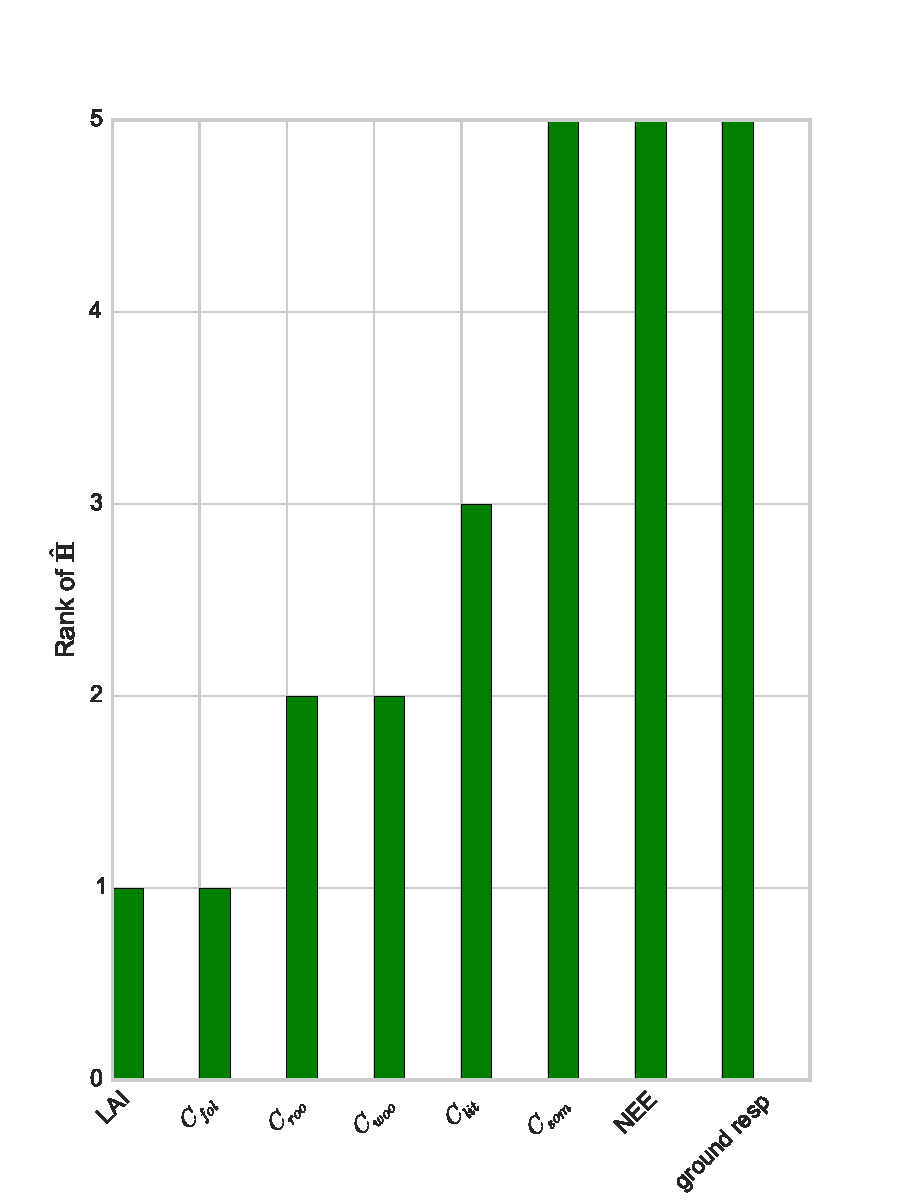
\includegraphics[width=0.5\textwidth]{chapter/chapter5/dalec1_obsrank.pdf}
    \caption{Rank of the observability matrix $\hat{\textbf{H}}$ for 5 observations of different types. The ranks shown here are computed analytically using SymPy \citep{Joyner:2012:OSC:2110170.2110185}.}
    \label{chap5:fig:D1_observability}
\end{figure}

From figure~\ref{chap5:fig:D1_observability} we can see that our system is observable for 5 observations of the soil and organic matter carbon pool $C_{som}$. In figure~\ref{chap5:fig:D1_observability} we have shown results for the rank of  $\hat{\textbf{H}}$ when we have 5 observations in each case; this has also been tested with increasing numbers of observations being added to the system with the results from figure~\ref{chap5:fig:D1_observability} remaining unchanged. 

The system being observable for observations of $C_{som}$ physically makes sense as all the carbon in the system that is not respired to the atmosphere eventually ends up in the soil and organic matter carbon pool, $C_{som}$, so that by taking observations of this pool we observe all the others. In a similar way $\hat{\textbf{H}}$ is also full rank for observations of NEE and ground respiration. We can see from the form of these observations in DALEC1 that they both contain indirect observations of $C_{som}$ with NEE taking the form
\begin{equation}
NEE^{i}=-(1-f_{auto})GPP^{i}(C_{fol}^{i-1}, \Psi) + \theta_{lit}C_{lit} e^{\Theta T^{i}} + \theta_{som}C_{som} e^{\Theta T^{i}} \label{chap5:eqn: D1_nee}
\end{equation}
with a corresponding linearised observation operator
\begin{equation}
\textbf{H}_{i} = \frac{\partial NEE^{i}}{\partial \textbf{x}_{i}} =
\begin{pmatrix}
-(1-f_{auto})\zeta^i & 0 & 0 & \theta_{lit} e^{\Theta T^{i}} & \theta_{som} e^{\Theta T^{i}}
\end{pmatrix},
\end{equation}
and for ground respiration
\begin{equation}
G_{resp}^{i}=\frac{1}{3}f_{auto}GPP^{i}(C_{fol}^{i-1}, \Psi) + \theta_{lit}C_{lit} e^{\Theta T^{i}} + \theta_{som}C_{som} e^{\Theta T^{i}} \label{chap5:neeeqn}
\end{equation}
(here we have assumed the fraction of total autotrophic respiration from below ground to be $\frac{1}{3}$) with a corresponding linearised observation operator
\begin{equation}
\textbf{H}_{i} = \frac{\partial G_{resp}^{i}}{\partial \textbf{x}_{i}} =
\begin{pmatrix}
\frac{1}{3}f_{auto}\zeta^i & 0 & 0 & \theta_{lit} e^{\Theta T^{i}} & \theta_{som} e^{\Theta T^{i}}
\end{pmatrix}.
\end{equation}
At flux tower sites NEE is the most observed quantity, these results give us confidence that we can construct a unique solution when working with flux tower data. We will further explore the concept of observability for the joint parameter and state estimation case with DALEC2 in section~\ref{chap5:sec: D2_observability}. 

%\FloatBarrier
\subsection{DALEC2 observability for state and parameter estimation} \label{chap5:sec: D2_observability}

For DALEC2 we perform joint parameter and state estimation and have an augmented state of size $n = 23$. The augmented state is made up of the 6 carbon pool state members and 17 model parameters as described in section~\ref{chap5:sec:dalec2}. As we are also estimating the parameters of DALEC2 the concept of observability for our system is closely linked to the concept of identifiability \citep{navon1998practical}. A system is identifiable if given observations of the state variables and knowledge of the model dynamics it is possible to obtain a unique deterministic set of model parameter values \citep{ljung1998system}. If a model parameter is not observable it will not be identifiable \citep{Jacquez1985}. It is therefore useful to compute the observability of the DALEC2 joint parameter and state estimation system.

We compute observability in the same way as in section~\ref{chap5:sec:D1observability} by finding the rank of $\hat{\textbf{H}}$ for a given set of observations. For the state and parameter estimation case we cannot compute the observability of the system analytically, it is therefore important to check that the numerical calculation of the rank of $\hat{\textbf{H}}$ for DALEC1 is equal to the rank when calculated analytically. This will give us confidence that our implementation of the numeric rank is correct for DALEC2 when applied to a well-conditioned problem as the implementation is the same in both cases. We have tested our numeric implementation for the state estimation case with DALEC1 and find the same results for the rank of $\hat{\textbf{H}}$ as for the analytic case, as shown in table~\ref{chap5:table: a_n_h_D1}. We calculate the rank of the $\hat{\textbf{H}}$ matrix using a singular value decomposition (SVD) which can have issues if the condition number of $\hat{\textbf{H}}$ is large \citep{Paige1981}. This is a problem we encounter in the DALEC2 case when trying to calculate the rank of $\hat{\textbf{H}}$ directly.  

\begin{table}[ht] 
\begin{center}
	\begin{tabular}{| l | l | l | l}
	\hline
	Observation & Rank of $\hat{\textbf{H}}$ (numeric) & Rank of $\hat{\textbf{H}}$ (analytic) \\ \hline
	LAI & 1 & 1 \\ \hline
	$C_{fol}$ & 1 & 1  \\ \hline
	$C_{roo}$ & 2 & 2 \\ \hline
	$C_{woo}$ & 2 & 2 \\ \hline
	$C_{lit}$ & 3 & 3 \\ \hline
	$C_{som}$ & 5 & 5 \\ \hline
	NEE & 5 & 5 \\ \hline
	$G_{resp}$ & 5 & 5 \\  
	\hline
	\end{tabular}
	\caption{Rank of $\hat{\textbf{H}}$ for 5 observations of different types for both numeric and analytic implementations with DALEC1.}
	\label{chap5:table: a_n_h_D1}
\end{center} 
\end{table}


\begin{figure}[ht]
    \centering
    \begin{subfigure}[b]{0.4\textwidth}
        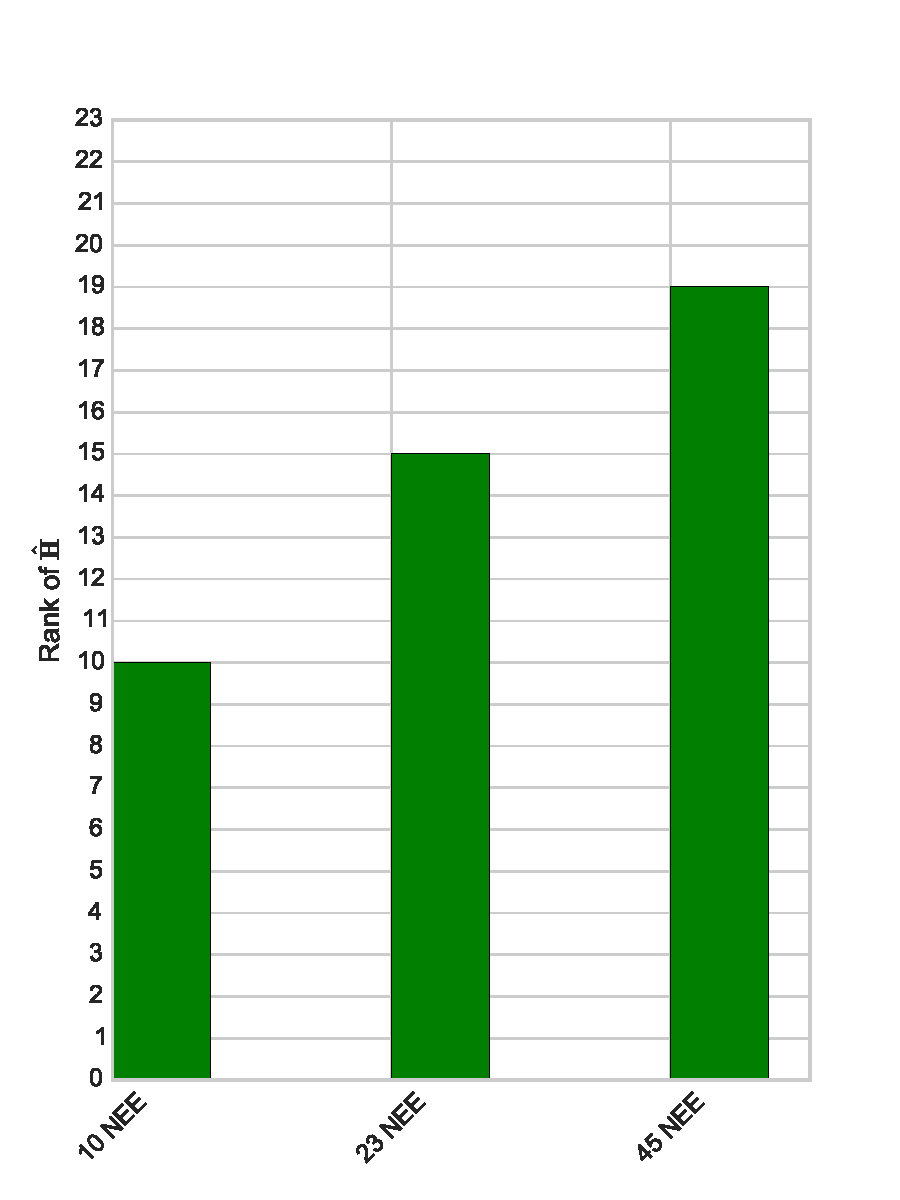
\includegraphics[width=\textwidth]{chapter/chapter5/dalec2_obsrank.pdf}
        \caption{Rank of $\hat{\textbf{H}}$}
        \label{chap5:fig:D2_observabilityrank}
    \end{subfigure}%
    \begin{subfigure}[b]{0.4\textwidth}
        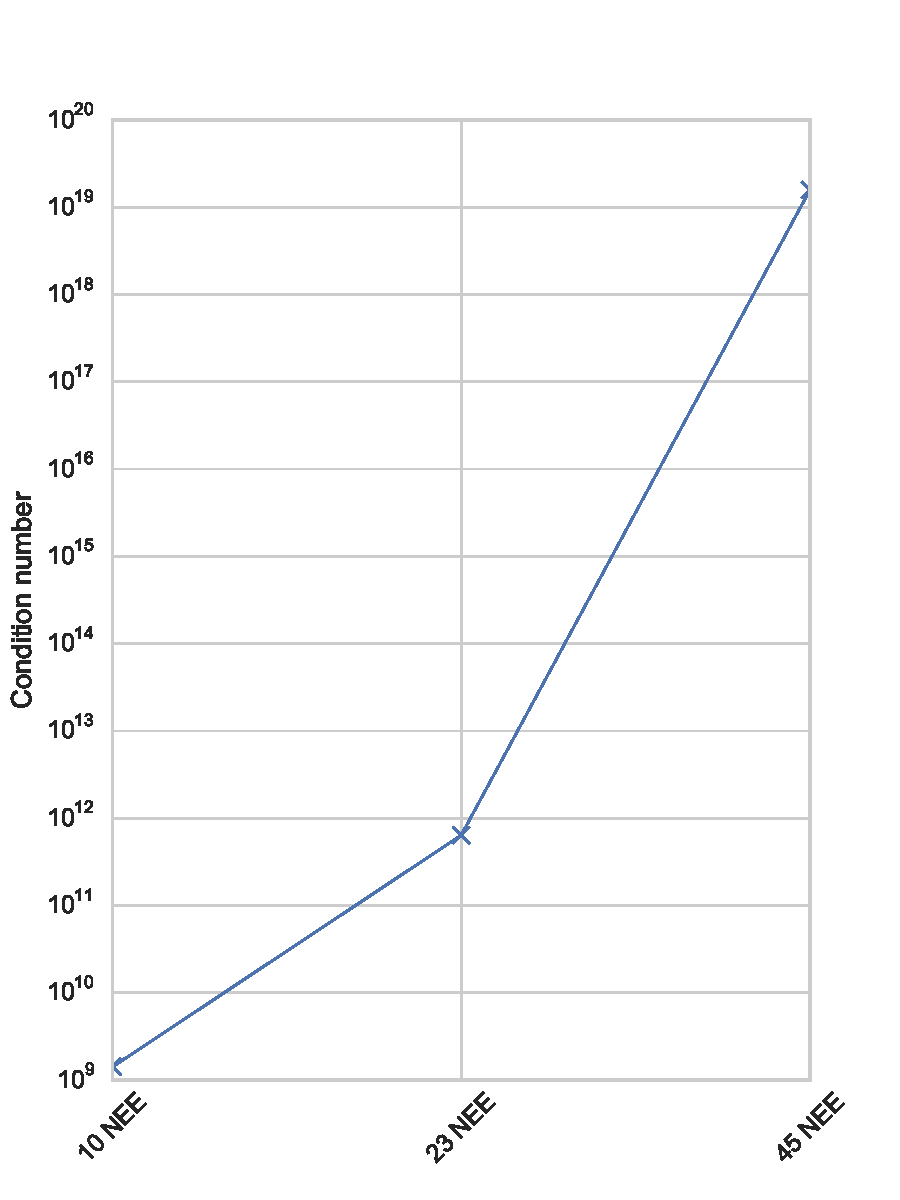
\includegraphics[width=\textwidth]{chapter/chapter5/dalec2_obsrankcond.pdf}
        \caption{Condition number of $\hat{\textbf{H}}$}
        \label{chap5:fig:D2_observabilitycond}
    \end{subfigure}
    \caption{Observability of DALEC2 for $\hat{\textbf{H}}$ with an increasing number of NEE observations displayed alongside the condition number for the $\hat{\textbf{H}}$ matrices.}
    \label{chap5:fig:D2_observability}
\end{figure}

Figure~\ref{chap5:fig:D2_observability} highlights the problems we have calculating the rank of the $\hat{\textbf{H}}$ matrix for the DALEC2 joint parameter and state estimation case. In figure~\ref{chap5:fig:D2_observabilityrank} we see that for 23 observations of NEE our system is unobservable as we have a rank deficient $\hat{\textbf{H}}$. However, we cannot trust the rank calculation of $\hat{\textbf{H}}$ in this case. Figure~\ref{chap5:fig:D2_observabilitycond} shows that for 23 observations of NEE, $\hat{\textbf{H}}$ has a condition number in the order of $10^{19}$. The condition number of a matrix corresponds to the ratio of the largest to the smallest singular values. A condition number of this size means that we have very small singular values. In the calculation of the rank of a matrix using an SVD we define the rank to be the number of singular values greater than the threshold \texttt{ tol = max(S) * max(n, m) * eps } \citep{press2007numerical}, where \texttt{S} is the vector of singular values, \texttt{n} and \texttt{m} are the rows and columns of the matrix whose rank we wish to calculate and \texttt{eps} is the machine accuracy for the datatype of \texttt{S} (In this case a double-precision float with \texttt{eps = 2.22e-16}). For 23 observations of NEE, $\hat{\textbf{H}}$ is classed as being rank deficient as \texttt{tol = 1.02e-10} and the three smallest singular values of $\hat{\textbf{H}}$ are \texttt{[1.39e-11, 7.84e-15, 1.46e-15]} but here we are working past the accuracy of the computer and so cannot have confidence that $\hat{\textbf{H}}$ is rank deficient in this case.

\begin{figure}[ht]
    \centering
    \begin{subfigure}[b]{0.4\textwidth}
        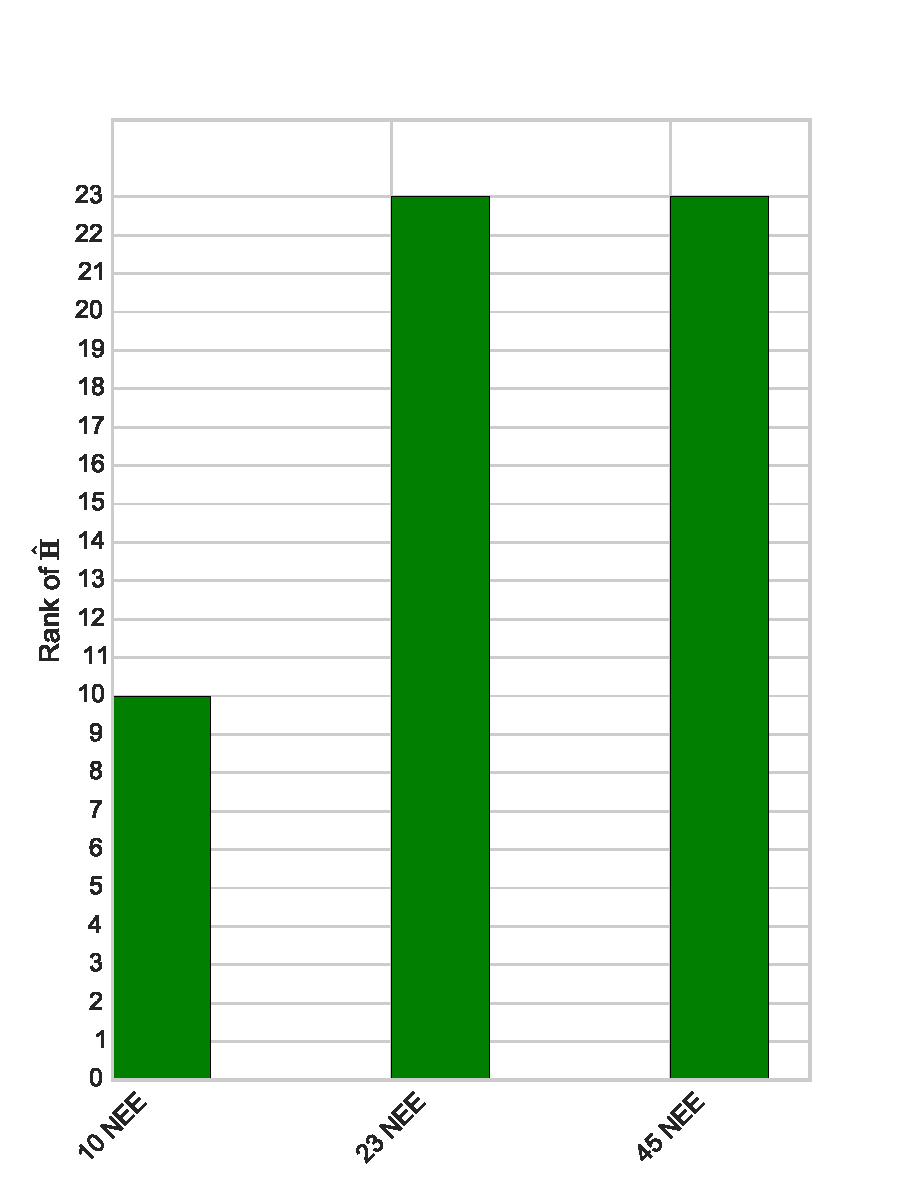
\includegraphics[width=\textwidth]{chapter/chapter5/dalec2_obsrankcvt.pdf}
        \caption{Rank of $\hat{\textbf{R}}^{-1/2}\hat{\textbf{H}}\textbf{D}^{1/2}$}
        \label{chap5:fig:D2_observailityrankcvt}
    \end{subfigure}
    \begin{subfigure}[b]{0.4\textwidth}
        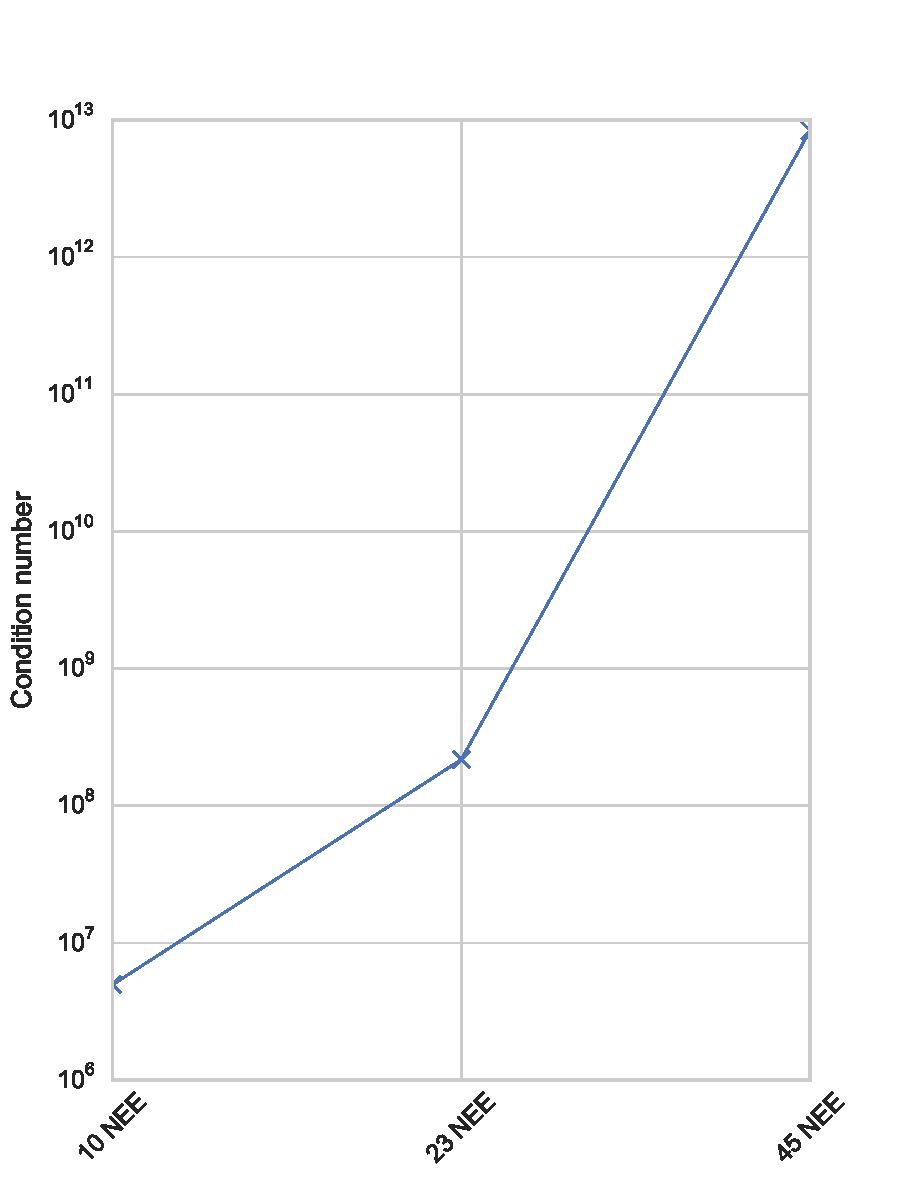
\includegraphics[width=\textwidth]{chapter/chapter5/dalec2_obsrankcvtcond.pdf}
        \caption{Condition number of $\hat{\textbf{R}}^{-1/2}\hat{\textbf{H}}\textbf{D}^{1/2}$}
        \label{chap5:fig:D2_observabilitycondcvt}
    \end{subfigure}
    \caption{Observability of the CVT DALEC2 for $\hat{\textbf{R}}^{-1/2}\hat{\textbf{H}}\textbf{D}^{1/2}$ with an increasing number of NEE observations displayed alongside the condition number for the $\hat{\textbf{R}}^{-1/2}\hat{\textbf{H}}\textbf{D}^{1/2}$ matrices.}
    \label{chap5:fig:D2_cvtobservability}
\end{figure}

In order to address the problem of ill-conditioning of the $\hat{\textbf{H}}$ matrix we can instead calculate the rank of the control variable transform observability matrix, $\hat{\textbf{R}}^{-1/2}\hat{\textbf{H}}\textbf{D}^{1/2}$, where the symbols have the same meaning as in section~\ref{chap3:sec:4dvar}, with $\textbf{D} = diag(\textbf{B})$. The rank of $\hat{\textbf{R}}^{-1/2}\hat{\textbf{H}}\textbf{D}^{1/2}$ and $\hat{\textbf{H}}$ are the same since $\hat{\textbf{R}}$ and $\textbf{D}$ are both full rank matrices. The results using this new better conditioned matrix are shown in Figure~\ref{chap5:fig:D2_cvtobservability}. From Figure~\ref{chap5:fig:D2_observabilitycondcvt} we can see this matrix is much better conditioned than $\hat{\textbf{H}}$, and for 23 observations of NEE we now have an observable system. Although the condition numbers here are still large we can have more confidence in these results as we are working within the precision of the computer.

\subsubsection{Observability for observations randomly distributed through time}

In the previous experiments we have considered increasing numbers of NEE observations taken on adjacent days. It is also useful to consider the observability of the system when we have a number of observations randomly distributed throughout a time window. This is more consistent with what we expect from the real data we have to work with.  

\begin{figure}[ht]
    \centering
    \begin{subfigure}[b]{0.4\textwidth}
        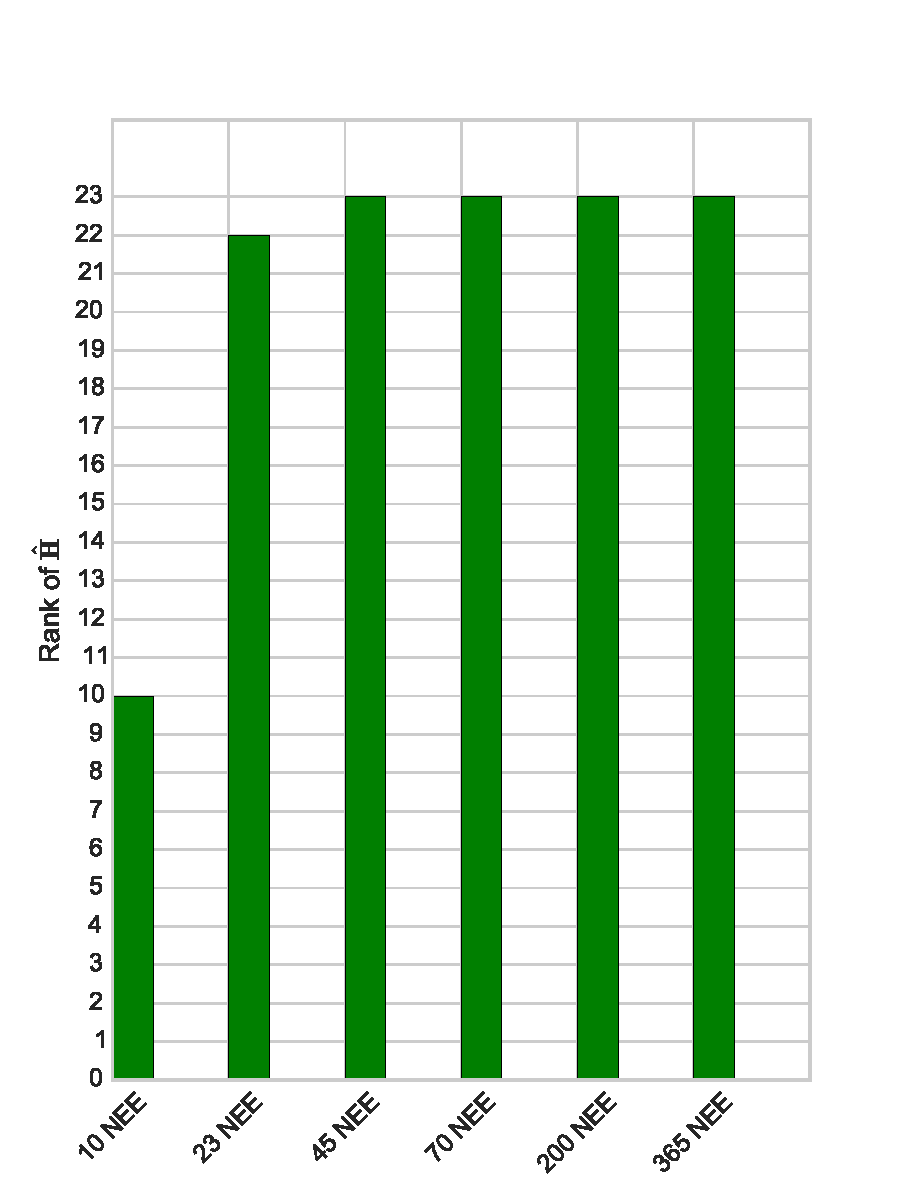
\includegraphics[width=\textwidth]{chapter/chapter5/dalec2_obsrankwind.pdf}
        \caption{Rank of $\hat{\textbf{H}}$}
        \label{chap5:fig:D2_observailityrankwind}
    \end{subfigure}
    \begin{subfigure}[b]{0.4\textwidth}
        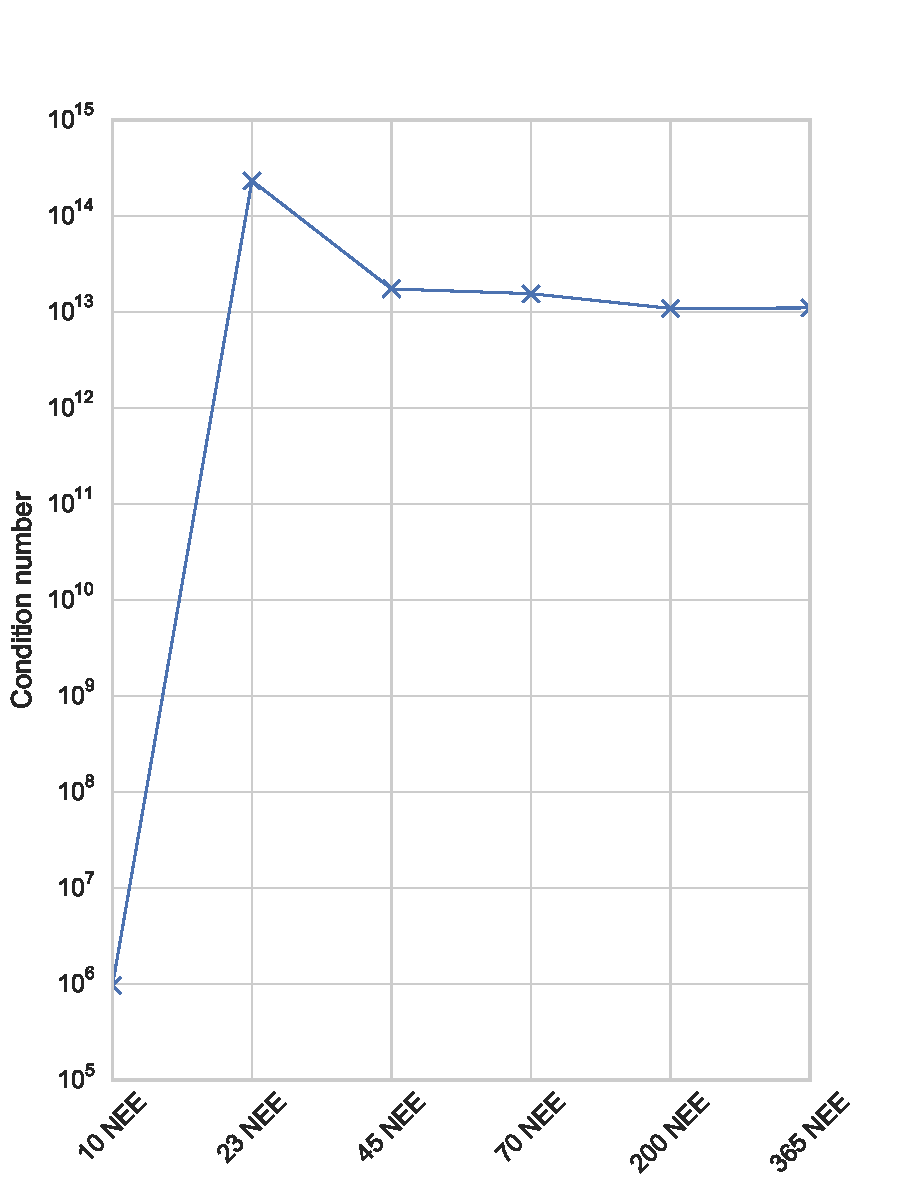
\includegraphics[width=\textwidth]{chapter/chapter5/dalec2_obsrankcondwind.pdf}
        \caption{Condition number of $\hat{\textbf{H}}$}
        \label{chap5:fig:D2_observabilitycondwind}
    \end{subfigure}
    \caption{Observability of DALEC2 for a $\hat{\textbf{H}}$ with an increasing number of NEE observations randomly distributed through a 1 year assimilation window (left). Condition number for the $\hat{\textbf{H}}$ matrices (right).}
    \label{chap5:fig:D2_observabilitywind}
\end{figure}

Figure~\ref{chap5:fig:D2_observabilitywind} shows the observability for an increasing number of observations distributed through a 1 year assimilation window. I this case we are using the matrix $\hat{\textbf{H}}$ and not the CVT observability matrix. In figure~\ref{chap5:fig:D2_observabilitywind} we see that having the observations randomly distributed throughout a 1 year assimilation window has improved the conditioning of $\hat{\textbf{H}}$ in comparison to figure~\ref{chap5:fig:D2_observability}. This is due to the observations being randomly distributed rather than adjacent. The rows of $\hat{\textbf{H}}$ are more distinct when being evolved to different times in the year by the tangent linear model rather than evolved to adjacent days only. However, we still have a rank deficient $\hat{\textbf{H}}$ for the 23 NEE observation case. From figure~\ref{chap5:fig:D2_observabilitycondwind} we see that this is the case where the condition number peaks. As we add more randomly distributed observations the condition number of $\hat{\textbf{H}}$ is reduced by an order of $10^{2}$ and we have a full rank $\hat{\textbf{H}}$. 

In figure~\ref{chap5:fig:D2_cvtobservabilitywind} we again see that using the CVT observability matrix has much improved the conditioning of the problem in comparison to figure~\ref{chap5:fig:D2_observabilitywind}. We now see that the DALEC2 system is observable when we have 23 observations of NEE randomly distributed throughout the 1 year assimilation window. We have more confidence that this is the case as the condition numbers for the CVT observability matrix are almost half the values of those for $\hat{\textbf{H}}$. We again see a similar pattern in figure~\ref{chap5:fig:D2_cvtobservabilitywind} for the condition numbers with a peak for 23 NEE observations and then a reduction of order $10^{2}$ when more observations are added. 

We have tested the observability of the system for observations of NEE when we have different driving data, linearising around different states and with different distributions of observations throughout our assimilation window and in every case we have an observable system given an adequate number of NEE observations (at least 23). We can therefore have confidence that for the available data, typically 60-80 observations of daily NEE for any year's window, we can construct a unique solution with the observations alone.

\begin{figure}[ht]
    \centering
    \begin{subfigure}[b]{0.4\textwidth}
        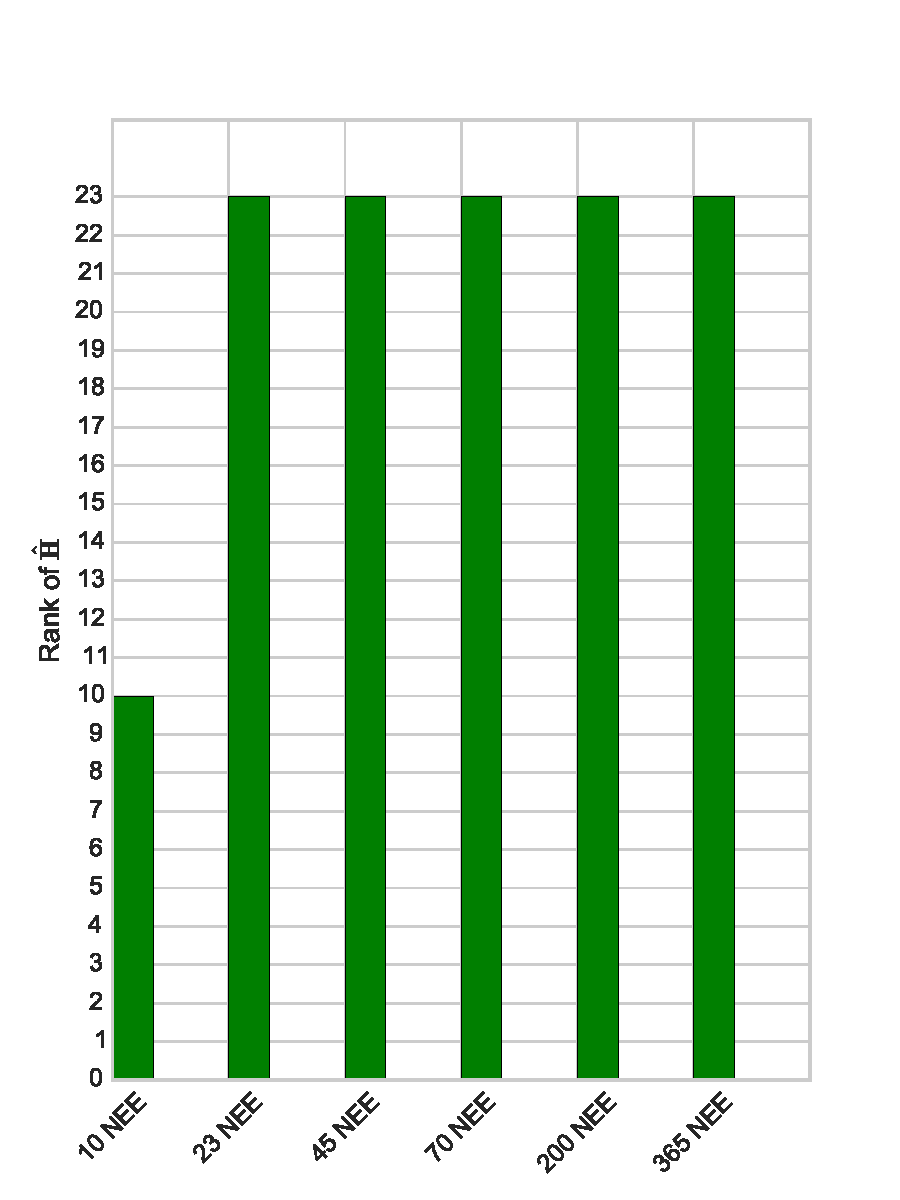
\includegraphics[width=\textwidth]{chapter/chapter5/dalec2_obsrankcvtwind.pdf}
        \caption{Rank of $\hat{\textbf{R}}^{-1/2}\hat{\textbf{H}}\textbf{D}^{1/2}$}
        \label{chap5:fig:D2_observailityrankcvtwind}
    \end{subfigure}
    \begin{subfigure}[b]{0.4\textwidth}
        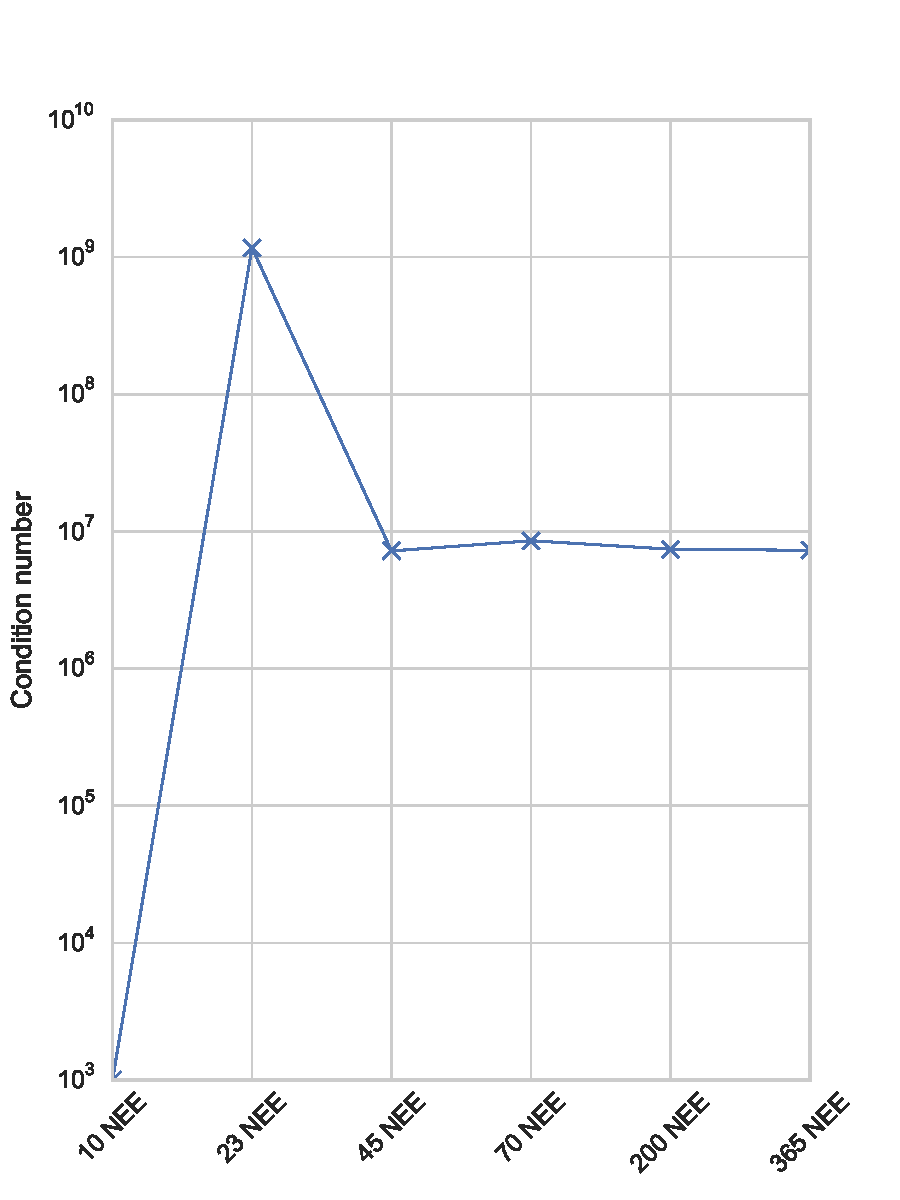
\includegraphics[width=\textwidth]{chapter/chapter5/dalec2_obsrankcondcvtwind.pdf}
        \caption{Condition number of $\hat{\textbf{R}}^{-1/2}\hat{\textbf{H}}\textbf{D}^{1/2}$}
        \label{chap5:fig:D2_observabilitycondcvtwind}
    \end{subfigure}
    \caption{Observability of the CVT DALEC2 system for $\hat{\textbf{R}}^{-1/2}\hat{\textbf{H}}\textbf{D}^{1/2}$ with an increasing number of NEE observations randomly distributed through a 1 year assimilation window (left). Condition number for the $\hat{\textbf{R}}^{-1/2}\hat{\textbf{H}}\textbf{D}^{1/2}$ matrices (right).}
    \label{chap5:fig:D2_cvtobservabilitywind}
\end{figure}


\subsection{DALEC1 information content for state estimation} \label{chap5:sec:D1_IC} %%%%%%%%%%%%%%%%%%% 
\subsubsection{Information content for a single observation} \label{chap5:sec:info_con_single_time}

For the DALEC1 state estimation we can calculate the analytic representation of the information content measures discussed in section~\ref{chap5:sec:IC}. This will allow us to understand how the information content changes for differing numbers of observations, different observation types and the effect of including observation error correlations in the assimilation scheme, before moving onto work with the larger DALEC2 joint parameter and state estimation case. For these experiments the elements of the state vector have corresponding background standard deviations $ \sigma_{cfol, b}, \sigma_{croo, b}, \sigma_{cwoo, b}, \sigma_{clit, b}, \sigma_{csom, b}$. We then have
\begin{equation}
\textbf{B} = \begin{pmatrix} 
\sigma_{cfol,b}^{2} & 0 & 0 & 0 & 0 \\
0 & \sigma_{croo,b}^{2} & 0 & 0 & 0 \\
0 & 0 & \sigma_{cwoo,b}^{2} & 0 & 0 \\
0 & 0 & 0 & \sigma_{clit,b}^{2} & 0 \\
0 & 0 & 0 & 0 & \sigma_{csom,b}^{2} \\
\end{pmatrix}. \label{chap5:eqn:BmatD1}
\end{equation}   

We begin by considering the Shannon Information Content (SIC) and degrees of freedom for signal (\(dfs\)) for a single observation of LAI. We have the linearised observation operator
\begin{equation}
\textbf{H}_{i} = \frac{\partial LAI^{i}}{\partial \textbf{x}_{i}} = \frac{\partial}{\partial \textbf{x}_{i}} \bigg( \frac{C_{fol}^{i}}{c_{lma}} \bigg) =
\begin{pmatrix}
\frac{1}{c_{lma}} & 0 & 0 & 0 & 0
\end{pmatrix}.
\end{equation}
As we have a single observation at one time, our observation error covariance matrix, $\bf{R}$, is just the variance of our observation of LAI at time $t_0$ ($\sigma_{LAI,o}^{2}$). Therefore,
\begin{equation}
\mathbf{R}_i=\sigma_{LAI,o}^{2}.
\end{equation}
We then have from equation~\eqref{chap3:eqn:a_cov_4dvar},
\begin{equation}
\begin{array} {lcl}
\mathbf{A} &=& (\mathbf{J}'')^{-1} \\
&=& (\mathbf{B}^{-1}+\hat{\mathbf{H}}^{T}\hat{\mathbf{R}}^{-1}\hat{\mathbf{H}})^{-1} \\
&=& (\mathbf{B}^{-1}+\mathbf{H}_0^{T}\mathbf{R}_0^{-1}\mathbf{H}_0)^{-1} \\
&=& \begin{pmatrix} 
\frac{c_{lma}^2 \sigma_{LAI,o}^2 \sigma_{cfol,b}^2}{\sigma_{cfol,b}^2 + c_{lma}^2 \sigma_{LAI,o}^2} & 0 & 0 & 0 & 0 \\
0 & \sigma_{croo,b}^{2} & 0 & 0 & 0 \\
0 & 0 & \sigma_{cwoo,b}^{2} & 0 & 0 \\
0 & 0 & 0 & \sigma_{clit,b}^{2} & 0 \\
0 & 0 & 0 & 0 & \sigma_{csom,b}^{2} \\
\end{pmatrix}.
\end{array}
\end{equation} 
We can now derive the SIC and $dfs$ using equation \eqref{chap5:eqn:sic} and \eqref{chap5:eqn:dfs} as,
\begin{equation}
\text{SIC} = \frac{1}{2}\text{ln}\frac{\begin{vmatrix} \mathbf{B} \end{vmatrix}}{\begin{vmatrix} \mathbf{A} \end{vmatrix}} = \frac{1}{2}\text{ln}\frac{(c_{lma}^2 \sigma_{LAI,o}^{2}+\sigma_{cfol,b}^{2})}{c_{lma}^2 \sigma_{LAI,o}^{2}}
=\frac{1}{2}\text{ln} \bigg(1+\frac{\sigma_{cfol,b}^{2}}{c_{lma}^2 \sigma_{LAI,o}^{2}}\bigg) \label{chap5:eqn:siclai}
\end{equation}
and 
\begin{equation}
dfs = n - tr(\textbf{B}^{-1}\textbf{A}) = 5 - \bigg(\frac{c_{lma}^2 \sigma_{LAI,o}^{2}}{(c_{lma}^2 \sigma_{LAI,o}^{2}+\sigma_{cfol,b}^{2})} + 4 \bigg) = 1 -\frac{c_{lma}^2 \sigma_{LAI,o}^{2}}{(c_{lma}^2 \sigma_{LAI,o}^{2}+\sigma_{cfol,b}^{2})}. \label{chap5:eqn:dfslai}
\end{equation}
We see that in general for a direct observation of any of the carbon pools $C$ we have
\begin{equation}
\text{SIC} =\frac{1}{2}\text{ln} \bigg(1+\frac{\sigma_{c,b}^{2}}{\sigma_{c,o}^{2}}\bigg) \label{chap5:eqn:sicC}
\end{equation}
and 
\begin{equation}
dfs = 1 -\frac{\sigma_{c,o}^{2}}{(\sigma_{c,o}^{2}+\sigma_{c,b}^{2})}, \label{chap5:eqn:dfsC}
\end{equation}
where $\sigma_{c,o}$ and $\sigma_{c,b}$ are the observation and background standard deviations respectively, corresponding to any of the 5 carbon pools.
We see the SIC for a single observation of one of the carbon pools is dependent on the ratio between the observation and background variances. The carbon pool observation which will give us the highest SIC is the observation with the largest ratio $\frac{\sigma_{c,b}^{2}}{\sigma_{c,o}^{2}}$. This is also the case for $dfs$. Assuming a fixed background standard deviation, the carbon pool observation which will give us the highest information content is the pool which we can measure most accurately, as expected. From equations~\eqref{chap5:eqn:siclai} and \eqref{chap5:eqn:dfslai} for an observation of LAI the information content is also dependent on $c_{lma}$ the parameter describing leaf mass area.

Next we consider the information content in a single observation of NEE. We have
\begin{equation}
\textbf{H}_{i} = \frac{\partial NEE^{i}}{\partial \textbf{x}_{i}} =
\begin{pmatrix}
-(1-f_{auto})\zeta^i & 0 & 0 & \theta_{lit} e^{\Theta T^{i}} & \theta_{som} e^{\Theta T^{i}}
\end{pmatrix}
\end{equation}
and
\begin{equation}
\mathbf{R}_i = \sigma_{NEE,o}^{2}.
\end{equation}
We then find
\begin{equation}
\text{SIC} = \frac{1}{2}\text{ln}\Bigg(1 + \frac{(f_{auto}-1)^{2}(\zeta^{i})^{2}\sigma_{cfol,b}^{2} + (e^{\Theta T^{i}})^2(\theta_{som}^2\sigma_{csom,b}^2+\theta_{lit}^2\sigma_{clit,b}^2)}{\sigma_{NEE,o}^{2}}\Bigg) \label{chap5:eqn:sicnee}
\end{equation}
and
\begin{equation}
dfs = 1 - \frac{\sigma_{NEE,o}^{2}}{(f_{auto}-1)^{2}(\zeta^{i})^{2}\sigma_{cfol,b}^{2}+(e^{\Theta T^{i}})^2(\theta_{som}^2\sigma_{csom,b}^2+\theta_{lit}^2\sigma_{clit,b}^2) +\sigma_{NEE,o}^{2}}. \label{chap5:eqn:dfsnee}
\end{equation}
We see that Equations~\eqref{chap5:eqn:sicnee} and \eqref{chap5:eqn:dfsnee} have a similar form to Equations~\eqref{chap5:eqn:sicC} and \eqref{chap5:eqn:dfsC}. The information content is again dependent on the ratio between the observation and background variances. The information content for the observations of NEE is also dependent on the magnitude of the first derivative of GPP with respect to \(C_{fol}\) and the magnitude of the exponential function of temperature controlling the rate of heterotrophic respiration, \(e^{\Theta T^{i}}\). Both the first derivative of GPP and  \(e^{\Theta T^{i}}\) will be of greater magnitude when we have higher mean daily temperatures. This means that observations of NEE made at times with higher temperatures will have higher information content and more of an impact on data assimilation results.
\begin{figure}[ht]
    \centering
    \begin{subfigure}[b]{0.45\textwidth}
        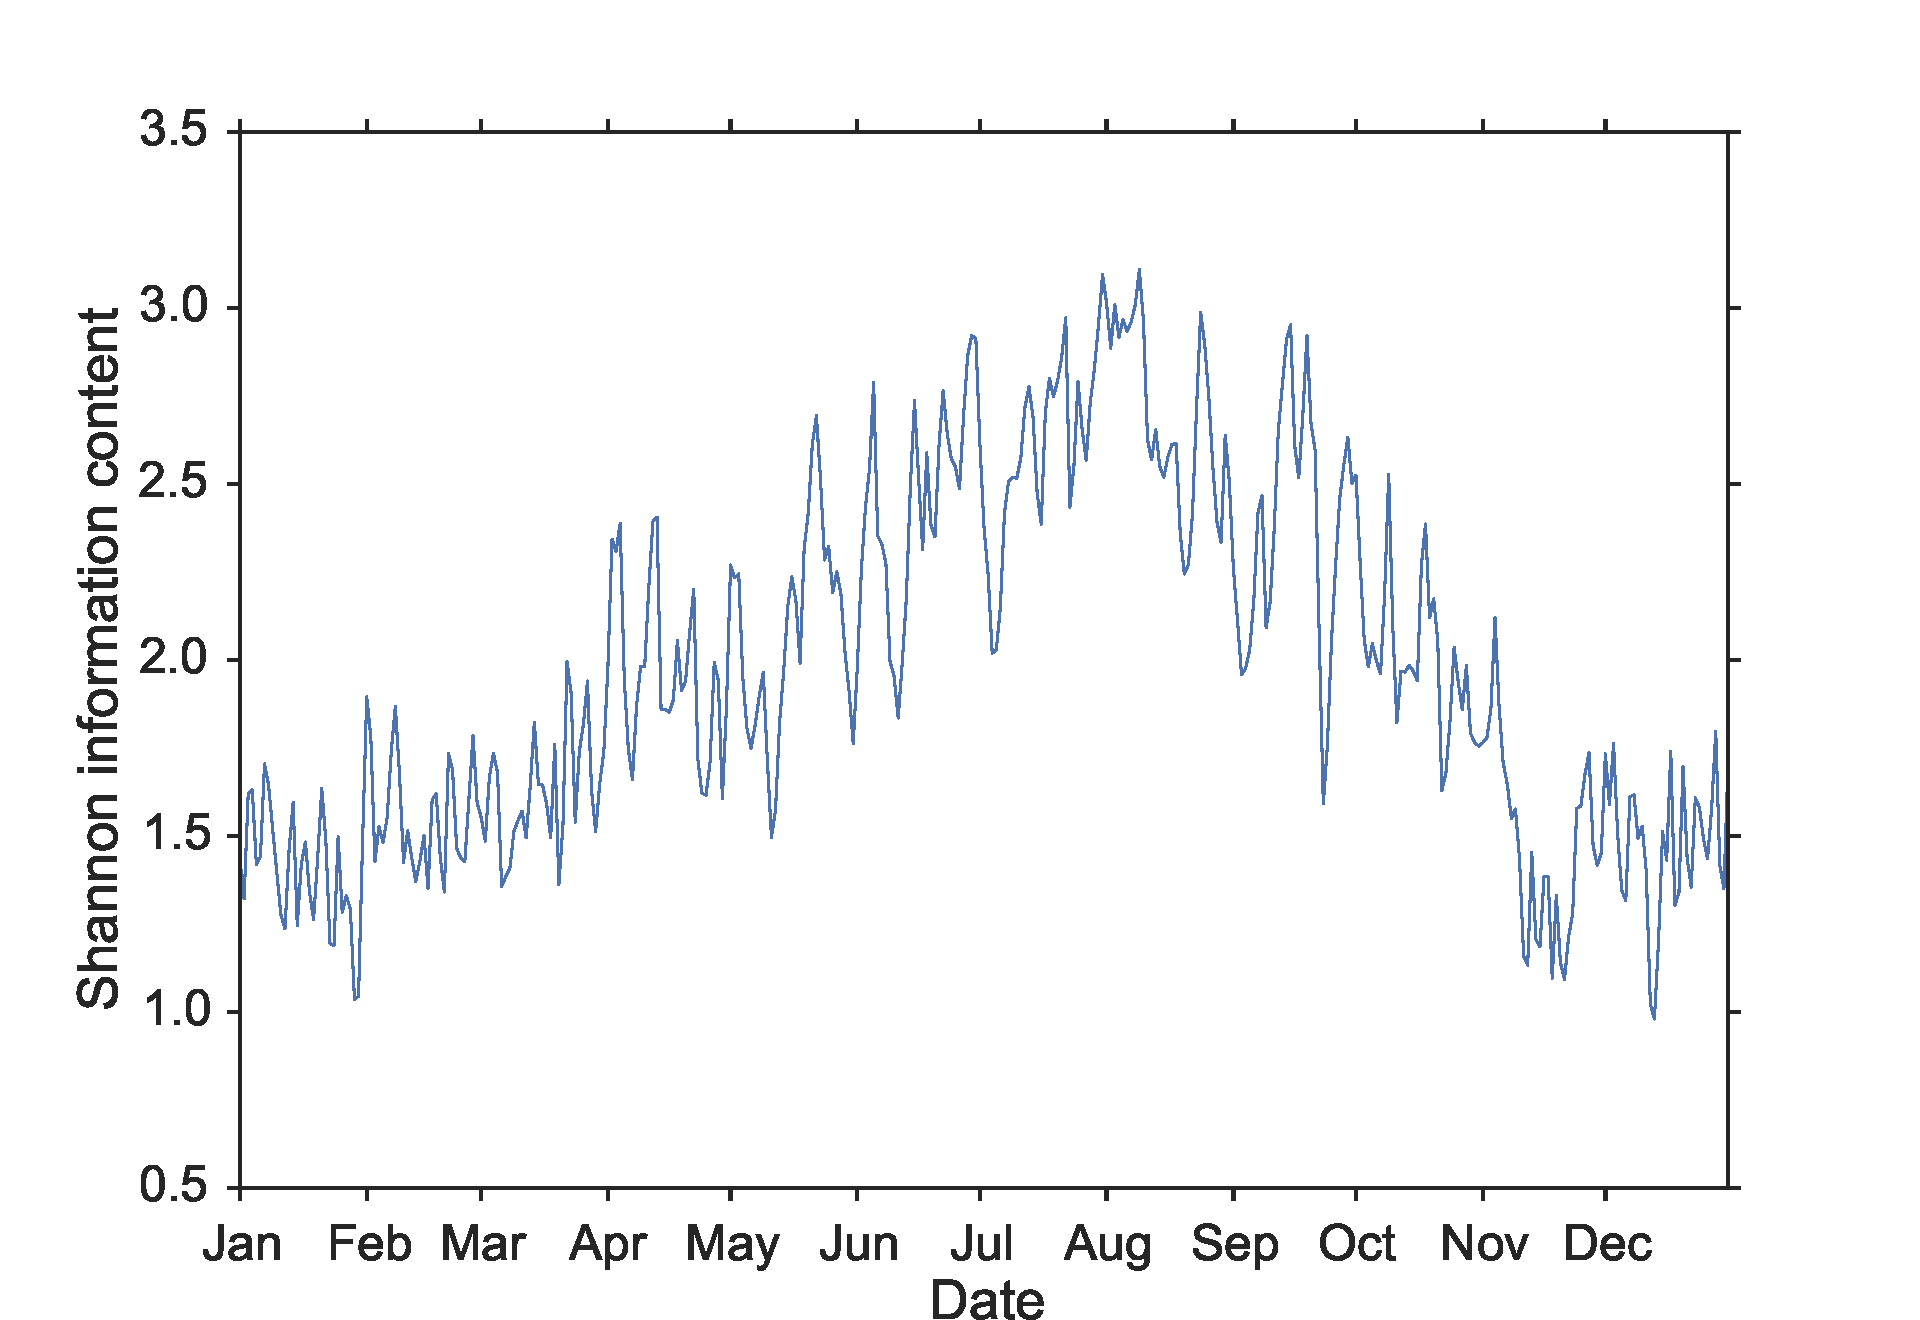
\includegraphics[width=\textwidth]{chapter/chapter5/oregon2007SICnee.pdf}
        \caption{SIC for single NEE observation}
        \label{chap5:fig:sic_nee_oregon2007}
    \end{subfigure}%
    \begin{subfigure}[b]{0.45\textwidth}
        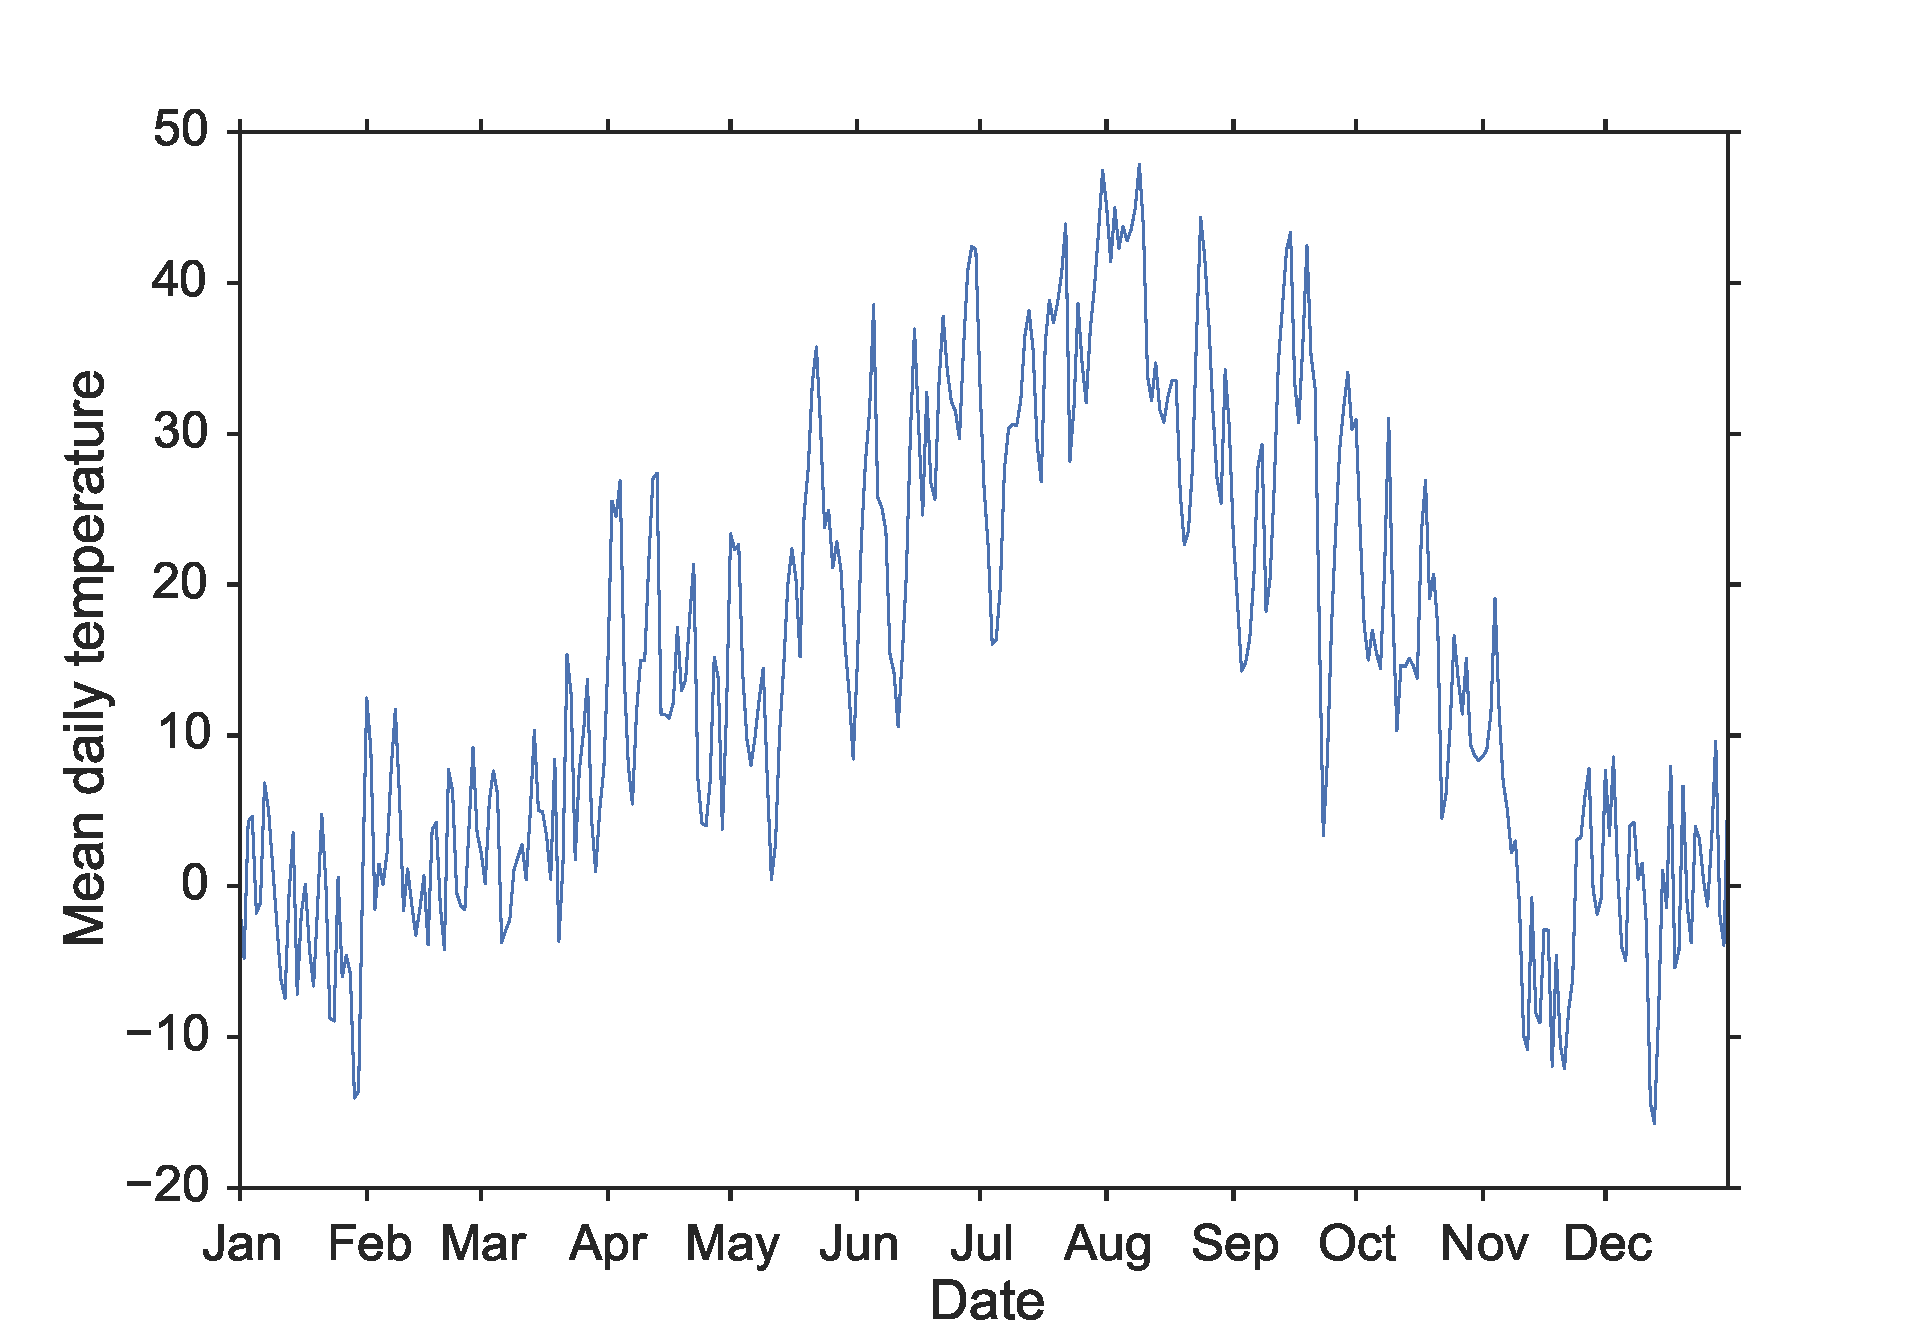
\includegraphics[width=\textwidth]{chapter/chapter5/oregon2007temp.pdf}
        \caption{Mean daily temperature for year's data}
        \label{chap5:fig:temp_nee_oregon2007}
    \end{subfigure}
    \caption{SIC for a single NEE observation changing throughout a year's window using driving data from a forest of ponderosa pine in Oregon taken in 2007 (left). Mean daily temperature for the same site and period (right).}
    \label{chap5:fig:neeSIC_temp_comp}
\end{figure}

In Figure~\ref{chap5:fig:neeSIC_temp_comp} we show how closely SIC is related to mean daily temperature for NEE observations throughout a year's window using daily driving data from a forest of ponderosa pine in Oregon (as described in section~\ref{chap5:sec:oregon}). Higher information content in summer observations of NEE makes physical sense. In summertime fluxes of carbon through the forest ecosystem are of greater magnitude than in winter, with more photosynthesis and respiration occurring. This gives us more information about the fluxes of carbon through our system in summertime observations of NEE. It is important to consider this result when planning for down time or routine maintenance at flux tower sites measuring NEE. The temperature dependence of information content will also hold true for other observations whose observation operators include the nonlinear temperature term controlling heterotrophic respiration. These observations include ground respiration, measured using soil respiration chambers, and total ecosystem respiration, estimated from nighttime NEE measurements.

In Figure~\ref{chap5:fig:sic_nee_oregon2007} we have assumed constant prior and observation standard deviations. This is an accurate assumption for our prior errors. However, it has been shown that NEE errors are heteroscedastic \citep{Richardson200838} and therefore scale with the magnitude of the flux. This would reduce the magnitude of the results shown in Figure~\ref{chap5:fig:sic_nee_oregon2007}, as our standard deviation in observations of summer NEE would be larger, reducing the information content.

For Figure~\ref{chap5:fig:sic_nee_oregon2007} we have used a numerical implementation in Python to calculate the SIC varying for 365 days of driving data. It is important to test our numerical implementation for correctness. In table~\ref{chap5:table:correctness_test} we show the SIC and \(dfs\) calculated both analytically and numerically. From this table we can see that both analytic and numerical implementations give us the same result to 15 or more significant figures. This gives us a degree of confidence that our implementation is also correct for DALEC2. In this table we have assumed constant prior and observation standard deviations for the carbon pools.

\begin{table}[ht] 
%\begin{center}
\centering
	\begin{tabular}{| l | l | l | l | l |}
	\hline
	Obs. & SIC analytic value & SIC numeric value & \(dfs\) analytic value & \(dfs\) numeric value \\ \hline
	NEE & 0.0209343224569909 & 0.0209343224569913 & 0.0410042587324008 & 0.0410042587324008 \\ \hline
	\(C_{fol}\) & 0.8047189562170501 & 0.8047189562170515 & 0.7999999999999998 & 0.7999999999999998 \\ \hline
	\(C_{roo}\) & 0.1838623900626585 & 0.1838623900626572 & 0.3076923076923075 & 0.3076923076923083 \\ \hline 	
	\(C_{woo}\)& 0.8047189562170501 & 0.8047189562170515 & 0.7999999999999998 & 0.7999999999999998 \\ \hline
	\(C_{lit}\) & 0.1838623900626585 & 0.1838623900626572 & 0.3076923076923075 & 0.3076923076923074 \\ \hline
	\(C_{som}\) & 0.1838623900626585 & 0.1838623900626572 & 0.3076923076923075 & 0.3076923076923074 \\
	\hline
	\end{tabular}
	\caption{Correctness tests showing numeric and analytic values of information content calculated using 2007 driving data and parameter values from an Oregon ponderosa pine forest.}
	\label{chap5:table:correctness_test}
%\end{center} 
\end{table}

\subsubsection{Information content for observations at a single time}

We next consider the SIC when we have more than one observation at a single time. Here we will investigate the representation of information content when assimilating an observation of NEE with an observation of a carbon pool state member. We begin with a single observation of NEE and an observation of \(C_{fol}\). We have the linearised observation operator,
\begin{equation}
\textbf{H}_{i} = \frac{\partial}{\partial \textbf{x}_{i}}\big(NEE^{i}, C_{fol}^{i} \big) =
 \begin{pmatrix}
-(1-f_{auto})\zeta^i & 0 & 0 & \theta_{lit} e^{\Theta T^{i}} & \theta_{som} e^{\Theta T^{i}}\\
1 & 0 & 0 & 0 & 0
\end{pmatrix}
\end{equation}
and observation error covariance matrix
\begin{equation}
\mathbf{R}_i = \begin{pmatrix}
\sigma_{NEE,o}^{2} & 0 \\
0 & \sigma_{cfol,o}^{2}
\end{pmatrix}.
\end{equation}
We then find,
\begin{equation}
\text{SIC} = \frac{1}{2}\text{ln} \Bigg( 1 + \frac{\sigma_{cfol,b}^{2}}{\sigma_{cfol,o}^{2}} + \frac{\xi^{i}}{\sigma_{NEE,o}^{2}} + \\
 \frac{\sigma_{cfol,b}^{2}(e^{\Theta T^{i}})^2(\theta_{som}^2\sigma_{csom,b}^2+\theta_{lit}^2\sigma_{clit,b}^2)}{\sigma_{NEE,o}^{2}\sigma_{cfol,o}^{2}} \Bigg) \label{chap5:eqn:sicneecfol}
 \end{equation}
 where, \( \xi^{i} = (f_{auto}-1)^{2}(\zeta^{i})^{2}\sigma_{cfol,b}^{2} + (e^{\Theta T^{i}})^2(\theta_{som}^2\sigma_{csom,b}^2+\theta_{lit}^2\sigma_{clit,b}^2) \). From equation~\eqref{chap5:eqn:sicneecfol} we can see that we have the first order terms for both NEE and \(C_{fol}\) as in equations~\eqref{chap5:eqn:sicC} and \eqref{chap5:eqn:sicnee}. We also have a second order term for the combination of these observations. We can repeat this for the other carbon pools and find for \(\textbf{H}_{i} = \frac{\partial}{\partial \textbf{x}_{i}}\big(NEE^{i}, C_{roo}^{i} \big) \),
\begin{equation}
\text{SIC} = \frac{1}{2}\text{ln} \Bigg( 1 + \frac{\sigma_{croo,b}^{2}}{\sigma_{croo,o}^{2}} + \frac{\xi^{i}}{\sigma_{NEE,o}^{2}} + \\
 \frac{\sigma_{croo,b}^{2}\big((f_{auto}-1)^{2}(\zeta^{i})^{2}\sigma_{cfol,b}^{2} + (e^{\Theta T^{i}})^2(\theta_{som}^2\sigma_{csom,b}^2+\theta_{lit}^2\sigma_{clit,b}^2)\big)}{\sigma_{NEE,o}^{2}\sigma_{croo,o}^{2}} \Bigg), \label{chap5:eqn:sicneecroo}
 \end{equation} 
for \(\textbf{H}_{i} = \frac{\partial}{\partial \textbf{x}_{i}}\big(NEE^{i}, C_{woo}^{i} \big) \),
\begin{equation}
\text{SIC} = \frac{1}{2}\text{ln} \Bigg( 1 + \frac{\sigma_{cwoo,b}^{2}}{\sigma_{cwoo,o}^{2}} + \frac{\xi^{i}}{\sigma_{NEE,o}^{2}} + \\
 \frac{\sigma_{cwoo,b}^{2}\big((f_{auto}-1)^{2}(\zeta^{i})^{2}\sigma_{cfol,b}^{2} + (e^{\Theta T^{i}})^2(\theta_{som}^2\sigma_{csom,b}^2+\theta_{lit}^2\sigma_{clit,b}^2)\big)}{\sigma_{NEE,o}^{2}\sigma_{cwoo,o}^{2}} \Bigg), \label{chap5:eqn:sicneecwoo}
 \end{equation}
 for \(\textbf{H}_{i} = \frac{\partial}{\partial \textbf{x}_{i}}\big(NEE^{i}, C_{lit}^{i} \big) \),
 \begin{equation}
\text{SIC} = \frac{1}{2}\text{ln} \Bigg( 1 + \frac{\sigma_{clit,b}^{2}}{\sigma_{clit,o}^{2}} + \frac{\xi^{i}}{\sigma_{NEE,o}^{2}} + \\
 \frac{\sigma_{clit,b}^{2}\big((f_{auto}-1)^{2}(\zeta^{i})^{2}\sigma_{cfol,b}^{2} + (e^{\Theta T^{i}})^2\theta_{som}^2\sigma_{csom,b}^2\big)}{\sigma_{NEE,o}^{2}\sigma_{clit,o}^{2}} \Bigg) \label{chap5:eqn:sicneeclit}
 \end{equation}
 and for \(\textbf{H}_{i} = \frac{\partial}{\partial \textbf{x}_{i}}\big(NEE^{i}, C_{som}^{i} \big) \),
 \begin{equation}
\text{SIC} = \frac{1}{2}\text{ln} \Bigg( 1 + \frac{\sigma_{csom,b}^{2}}{\sigma_{csom,o}^{2}} + \frac{\xi^{i}}{\sigma_{NEE,o}^{2}} + \\
 \frac{\sigma_{csom,b}^{2}\big((f_{auto}-1)^{2}(\zeta^{i})^{2}\sigma_{cfol,b}^{2} + (e^{\Theta T^{i}})^2\theta_{lit}^2\sigma_{clit,b}^2\big)}{\sigma_{NEE,o}^{2}\sigma_{csom,o}^{2}} \Bigg). \label{chap5:eqn:sicneecsom}
 \end{equation}
Assuming constant prior and observation standard deviations across our carbon pool observations we see that the information content will be largest in equations~\eqref{chap5:eqn:sicneecroo} and \eqref{chap5:eqn:sicneecwoo}. For both \(\textbf{H}_{i} = \frac{\partial}{\partial \textbf{x}_{i}}\big(NEE^{i}, C_{roo}^{i} \big) \) and \(\textbf{H}_{i} = \frac{\partial}{\partial \textbf{x}_{i}}\big(NEE^{i}, C_{woo}^{i} \big) \) we have an extra term in the numerator for our second order term corresponding to the combination of the two observations. If we consider the linearised observation operator for both these cases,
\begin{equation}
\textbf{H}_{i} = \frac{\partial}{\partial \textbf{x}_{i}}\big(NEE^{i}, C_{roo}^{i} \big) =
 \begin{pmatrix}
-(1-f_{auto})\zeta^i & 0 & 0 & \theta_{lit} e^{\Theta T^{i}} & \theta_{som} e^{\Theta T^{i}}\\
0 & 1 & 0 & 0 & 0
\end{pmatrix}
\end{equation}
and
\begin{equation}
\textbf{H}_{i} = \frac{\partial}{\partial \textbf{x}_{i}}\big(NEE^{i}, C_{woo}^{i} \big) =
 \begin{pmatrix}
-(1-f_{auto})\zeta^i & 0 & 0 & \theta_{lit} e^{\Theta T^{i}} & \theta_{som} e^{\Theta T^{i}}\\
0 & 0 & 1 & 0 & 0
\end{pmatrix},
\end{equation}
we can see that these observations provide an orthogonal constraint to the observation of NEE. Neither of these pools are observed with a single observation of NEE. The information content being greater when assimilating \(C_{roo}\) or \(C_{woo}\) alongside NEE is therefore expected. 

In practice we cannot assume constant prior and observation errors across the different carbon pools. Root carbon is hard to measure accurately \citep{brown2002measuring}. However, woody biomass (\(C_{woo}\)) is regularly measured using mensuration \citep{husch2002forest} or point-centred quarter methods \citep{dahdouh2006empirical} at forest sites. Advancements in Light Detection And Ranging (LiDAR) scanning \citep{Lefsky199983} mean that we have increasingly more accurate observations of woody biomass. The European Space Agency BIOMASS mission \citep{le2011biomass} will also provide a much more abundant source of woody biomass measurements in the future. If we consider NEE to be the main observation currently used in ecosystem data assimilation, then the increasing number of available woody biomass measurements will benefit assimilation schemes greatly.

\subsubsection{Information content in successive observations} \label{chap5:sec:D1_succ_obs}

In section~\ref{chap5:sec:info_con_single_time} we investigate the information in observation for DALEC1 at a single time. In this section we will consider successive observations in time. It has been shown that the SIC in observations is additive with successive observations in time. The proof for this can be found in appendix A.1 of \citet{Fowler2012}. We can see this if we calculate the SIC for successive observations of foliar carbon, \(C_{fol}\). We have the linearised observation operator and observation error covariance matrix at time $t_i$,
\begin{equation}
\mathbf{H}_{i} = \frac{\partial C_{fol}^{i}}{\partial \textbf{x}_i} = \begin{pmatrix}
1 & 0 & 0 & 0 & 0
\end{pmatrix}
\hspace{5mm} \text{and} \hspace{5mm}
\mathbf{R}_i=\sigma_{cfol,o}^{2}.
\end{equation}
For two successive observations of \(C_{fol}\) we have,
\begin{equation}
\hat{\mathbf{H}}=
\begin{pmatrix}
\mathbf{H}_0 \\
\mathbf{H}_1\mathbf{M}_0\\
\end{pmatrix}
=
\begin{pmatrix}
1 & 0 & 0 & 0 & 0 \\
(1-\theta_{fol})+f_{fol}(1-f_{auto})\zeta^0 & 0 & 0 & 0 & 0\\
\end{pmatrix}
\end{equation}
and
\begin{equation}
\hat{\mathbf{R}}=
\begin{pmatrix}
\mathbf{R}_0 & 0  \\
0 & \mathbf{R}_1  \\
\end{pmatrix}
=
\begin{pmatrix}
\sigma_{cfol,o}^{2} & 0  \\
0 & \sigma_{cfol,o}^{2}  \\
\end{pmatrix}.
\end{equation}
We then have,
\begin{equation}
SIC = \frac{1}{2}\text{ln}\frac{\begin{vmatrix} \mathbf{B} \end{vmatrix}}{\begin{vmatrix} \mathbf{A} \end{vmatrix}} =\frac{1}{2}\text{ln} \bigg(1+\frac{\sigma_{cfol,b}^{2}}{\sigma_{cfol,o}^{2}}+\frac{\sigma_{cfol,b}^{2}\eta_0^{2}}{\sigma_{cfol,o}^{2}} \bigg), \label{chap5:eq:sic_2cfol}
\end{equation}
where $\eta_i=(1-\theta_{fol})+f_{fol}(1-f_{auto})\zeta^{i}$. We see this is similar to equation~\eqref{chap5:eqn:sicC} for the SIC of a single carbon pool observation but with an added term evolved by the linearised model. Here the second term is multiplied by \(\eta_{0}^2\) which is the square of the first element of the linearised model \(\mathbf{M}_0\). We can continue adding more observations at successive times. For three observations at successive times we have,
\begin{equation}
SIC =\frac{1}{2}\text{ln} \bigg(1+\frac{\sigma_{cfol,b}^{2}}{\sigma_{cfol,o}^{2}}+\frac{\sigma_{cfol,b}^{2}\eta_0^{2}}{\sigma_{cfol,o}^{2}}+\frac{\sigma_{cfol,b}^{2}\eta_0^{2}\eta_1^{2}}{\sigma_{cfol,o}^{2}} \bigg),
\end{equation}
for four,
\begin{equation}
SIC =\frac{1}{2}\text{ln} \bigg(1+\frac{\sigma_{cfol,b}^{2}}{\sigma_{cfol,o}^{2}}+\frac{\sigma_{cfol,b}^{2}\eta_0^{2}}{\sigma_{cfol,o}^{2}}+\frac{\sigma_{cfol,b}^{2}\eta_0^{2}\eta_1^{2}}{\sigma_{cfol,o}^{2}}+\frac{\sigma_{cfol,b}^{2}\eta_0^{2}\eta_1^{2}\eta_2^{2}}{\sigma_{cfol,o}^{2}} \bigg).
\end{equation}
Using a simple proof by induction we find that for \(n\) successive observations we have,
\begin{equation}
SIC\text{ for }n\text{ successive observations of }C_{fol} = \frac{1}{2}\text{ln}\bigg(1+\frac{\sigma_{cfol,b}^{2}}{\sigma_{cfol,o}^{2}}\big(1+\sum_{k=0}^{n-2}\prod_{i=0}^{k}\eta_i^{2}\big)\bigg)
\end{equation}
This demonstrates that SIC is additive for successive observations in time. In Figure~\ref{chap5:fig:ic_succ_cf} we have plotted the SIC and \(dfs\) for increasing numbers of observations of \(C_{fol}\), using a year of meteorological driving data from a pine stand in Oregon. We see that as successive observations are added the information content tends to a limit where we are adding no new information with extra observations of \(C_{fol}\). For \(dfs\) this limit is one as we are only observing a single degree of freedom so cannot constrain more than a single element of the state. For SIC we add a decreasing amount of information as observations are made further away from the initial state. We find similar results for all other carbon pools. This suggests making observations of any individual carbon pool for a forest site too often is not cost effective as after just a few observations the information you are adding to your system begins to decrease. 

\begin{figure}[ht]
    \centering
    \begin{subfigure}[b]{0.45\textwidth}
        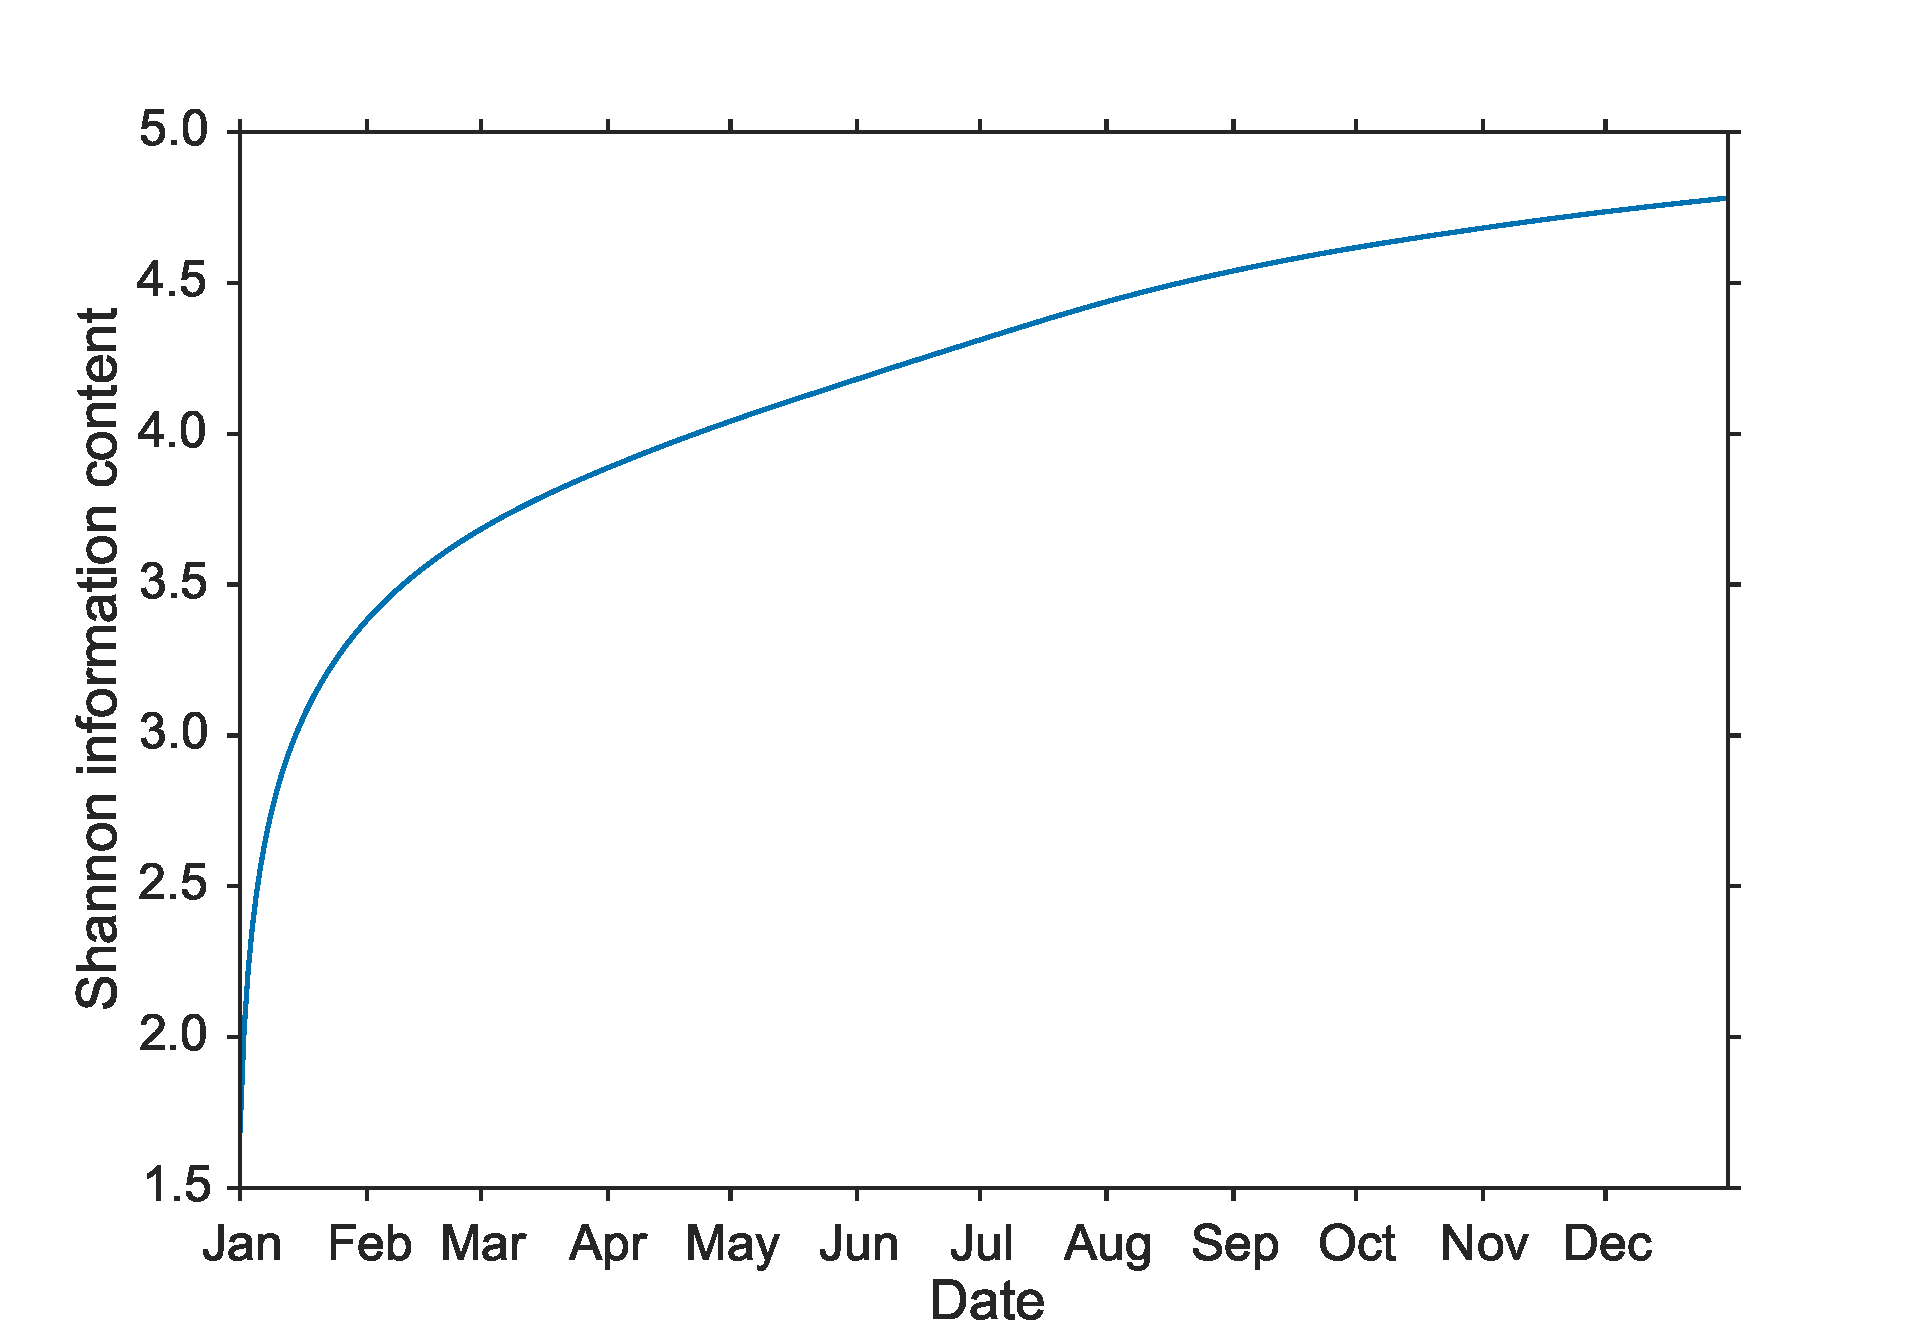
\includegraphics[width=\textwidth]{chapter/chapter5/sic_succ_cf.pdf}
        \caption{SIC for successive \(C_{fol}\) observations}
        \label{chap5:fig:sic_succ_cf}
    \end{subfigure}%
    \begin{subfigure}[b]{0.45\textwidth}
        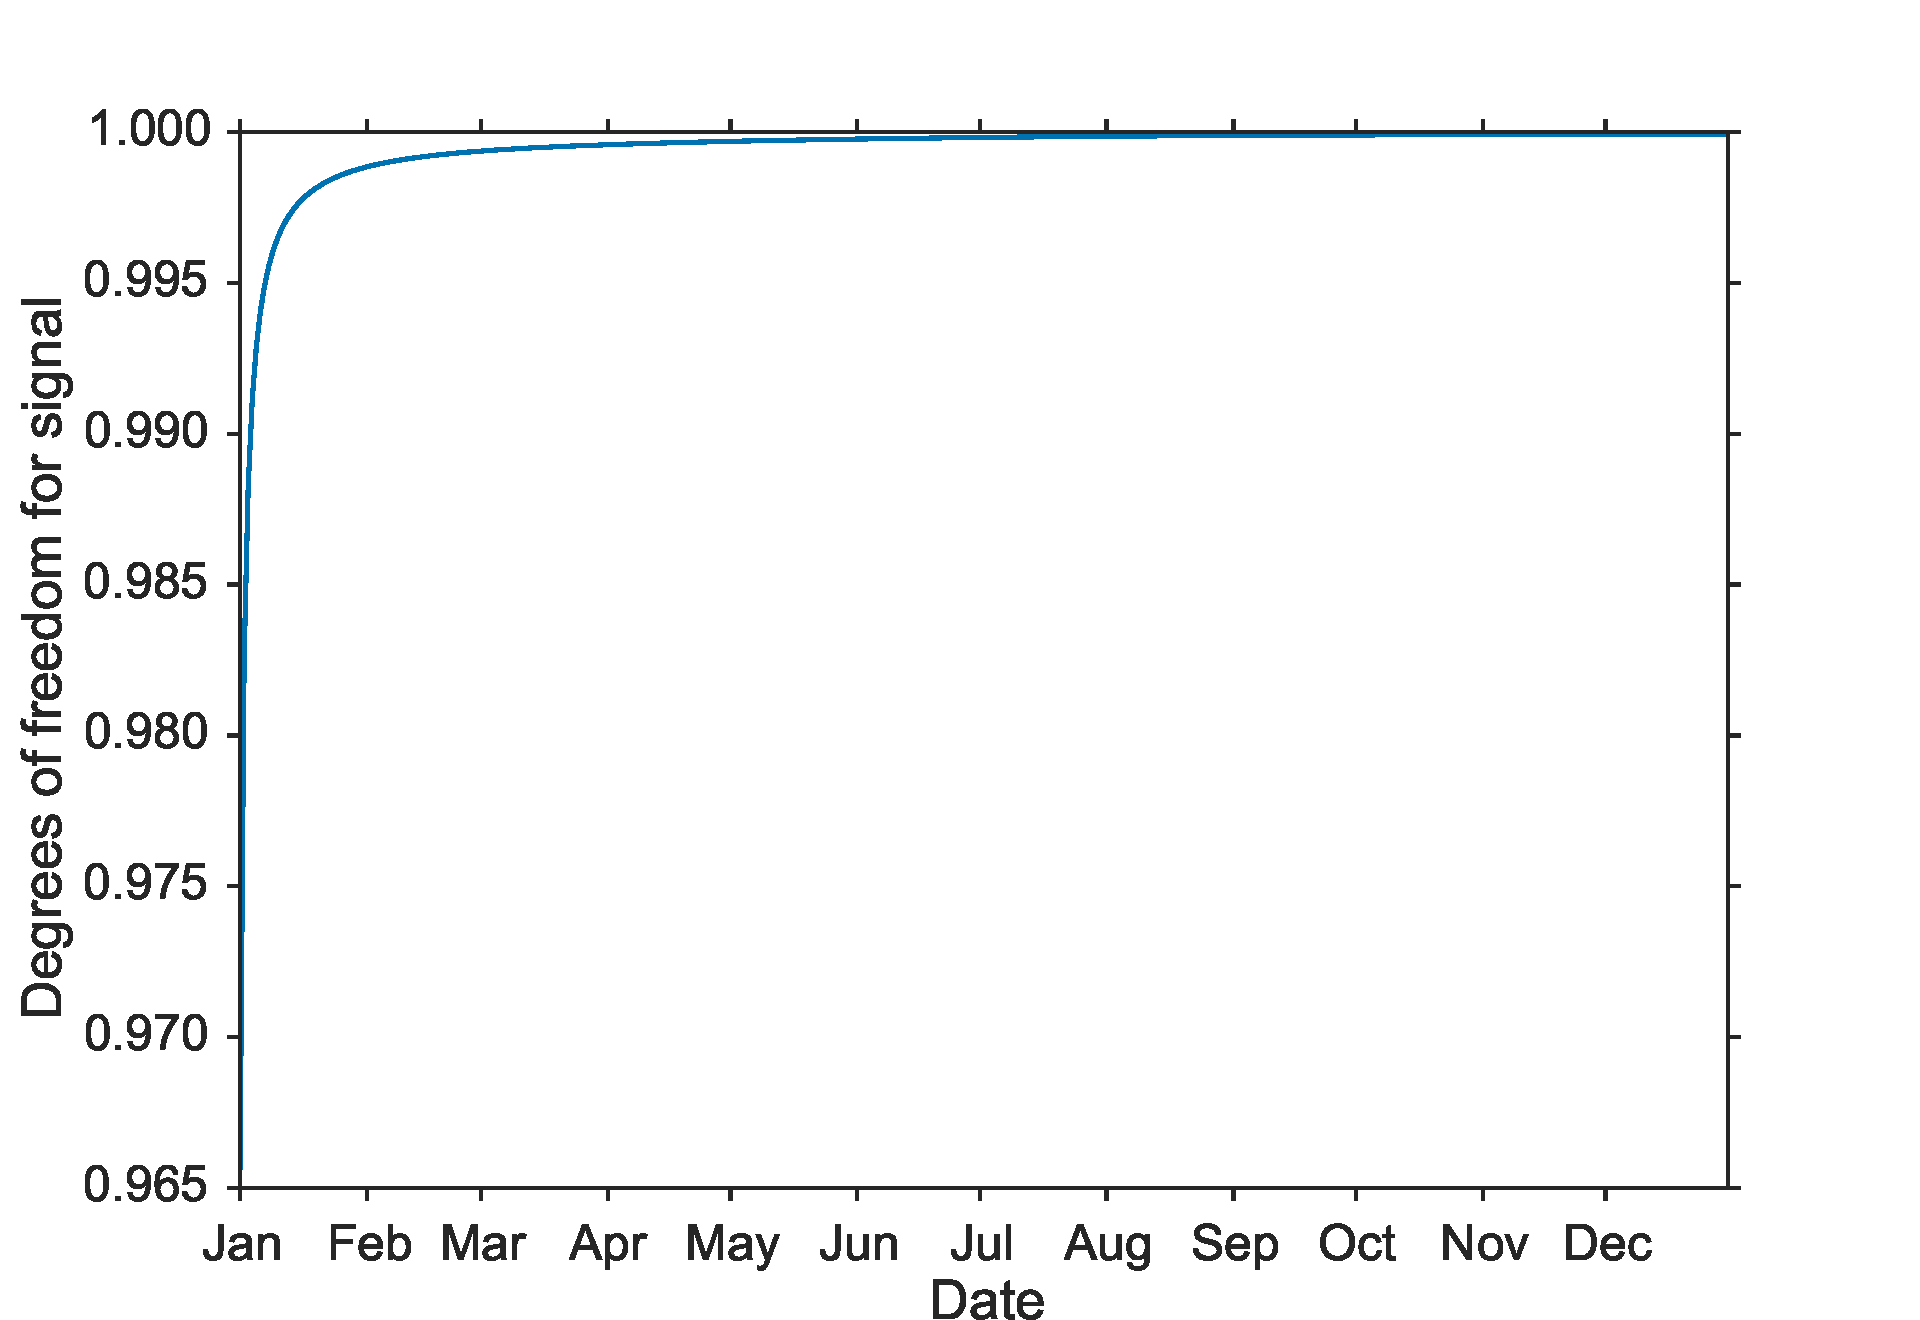
\includegraphics[width=\textwidth]{chapter/chapter5/dfs_succ_cf.pdf}
        \caption{\(dfs\) for successive \(C_{fol}\) observations}
        \label{chap5:fig:dfs_succ_cf}
    \end{subfigure}
    \caption{SIC and \(dfs\) for as successive \(C_{fol}\) observations are added throughout a year's window using driving data from a pine stand in Oregon taken in 2007.}
    \label{chap5:fig:ic_succ_cf}
\end{figure}

In section~\ref{chap5:sec:info_con_single_time} it was shown that observations of NEE made during the summer had significantly higher information content than those made during winter for an evergreen forest site. In figure~\ref{chap5:fig:ic_succ_nee} we show that 27 days of successive winter NEE observations (made from January \(1^{\text{st}}\) 2007) are required to give the same information content as a single summer observation of NEE (taken on \( 22^{\text{nd}} \) June 2007).

\begin{figure}[ht]
    \centering
    \begin{subfigure}[b]{0.45\textwidth}
        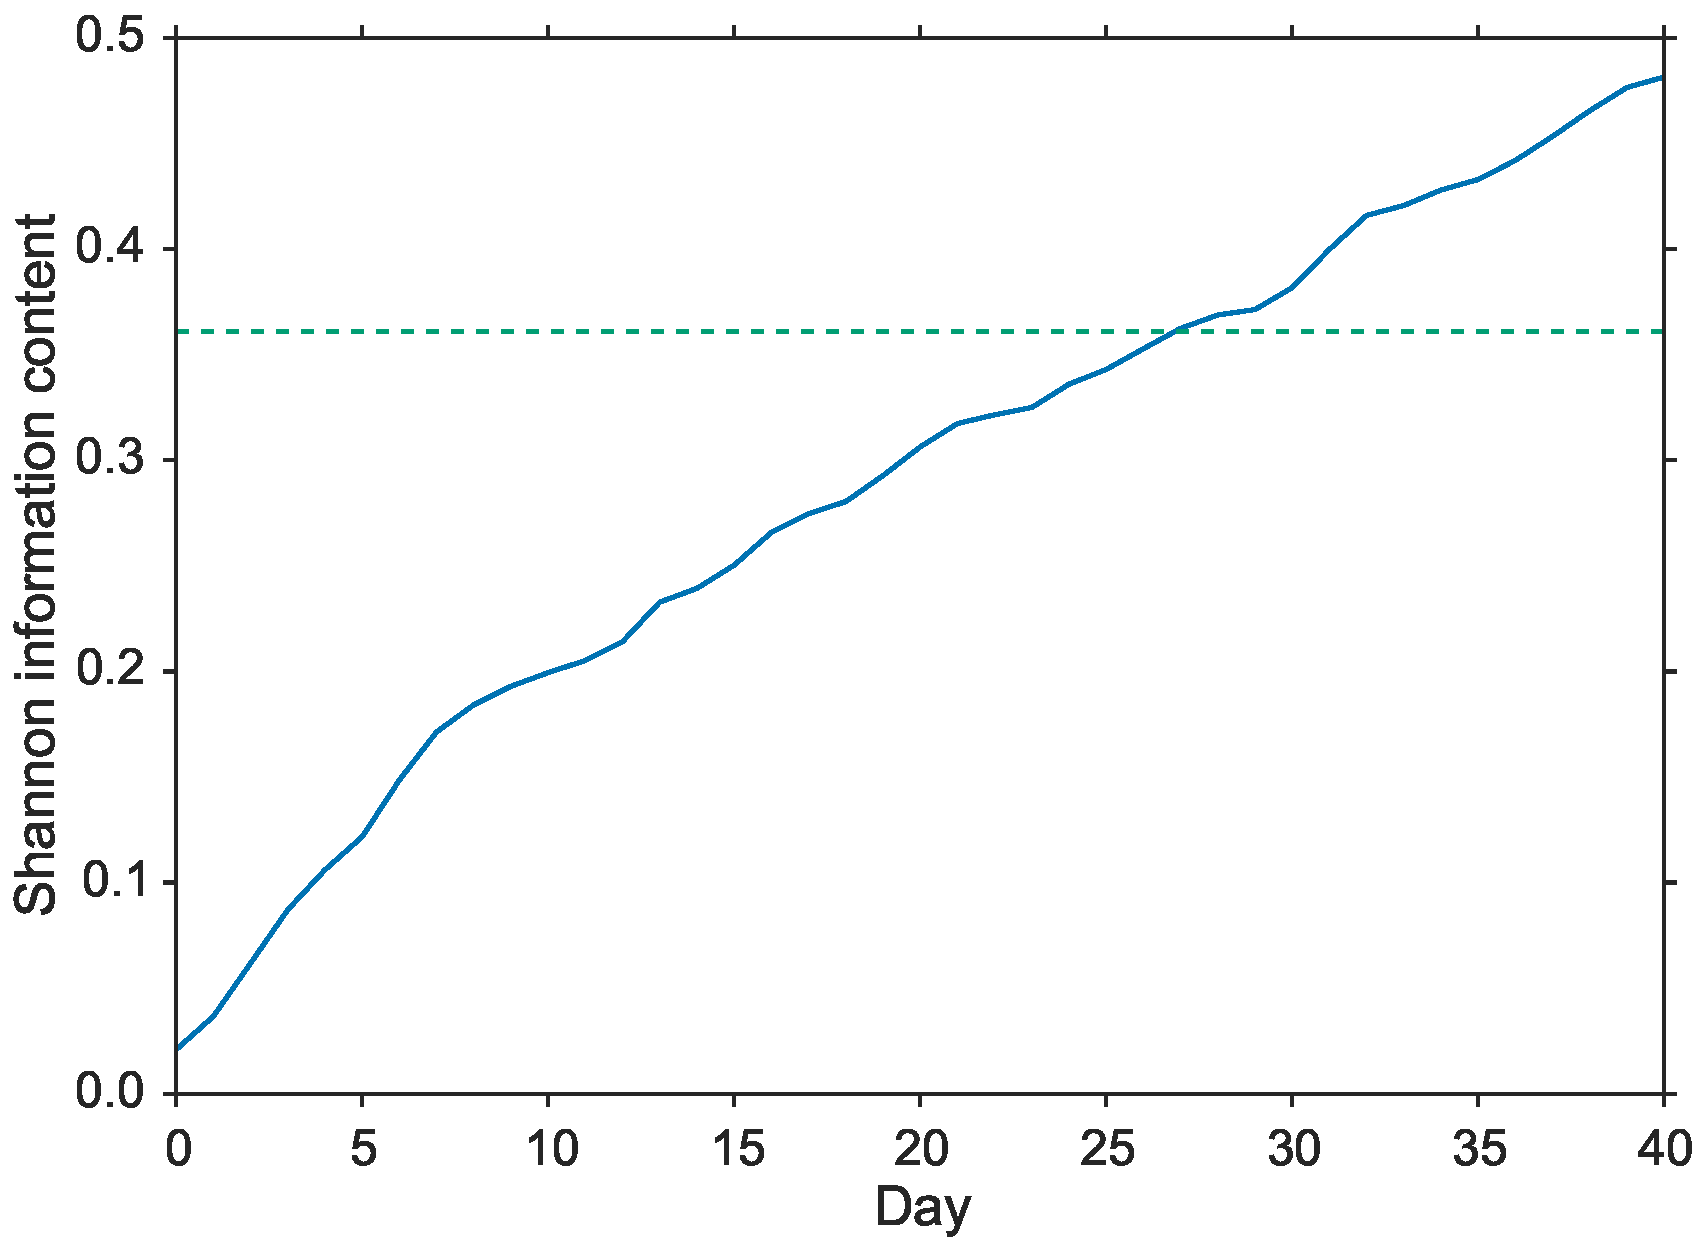
\includegraphics[width=\textwidth]{chapter/chapter5/sic_succ_nee.pdf}
        \caption{SIC for successive NEE observations}
        \label{chap5:fig:sic_succ_nee}
    \end{subfigure} \hspace{5mm}
    \begin{subfigure}[b]{0.45\textwidth}
        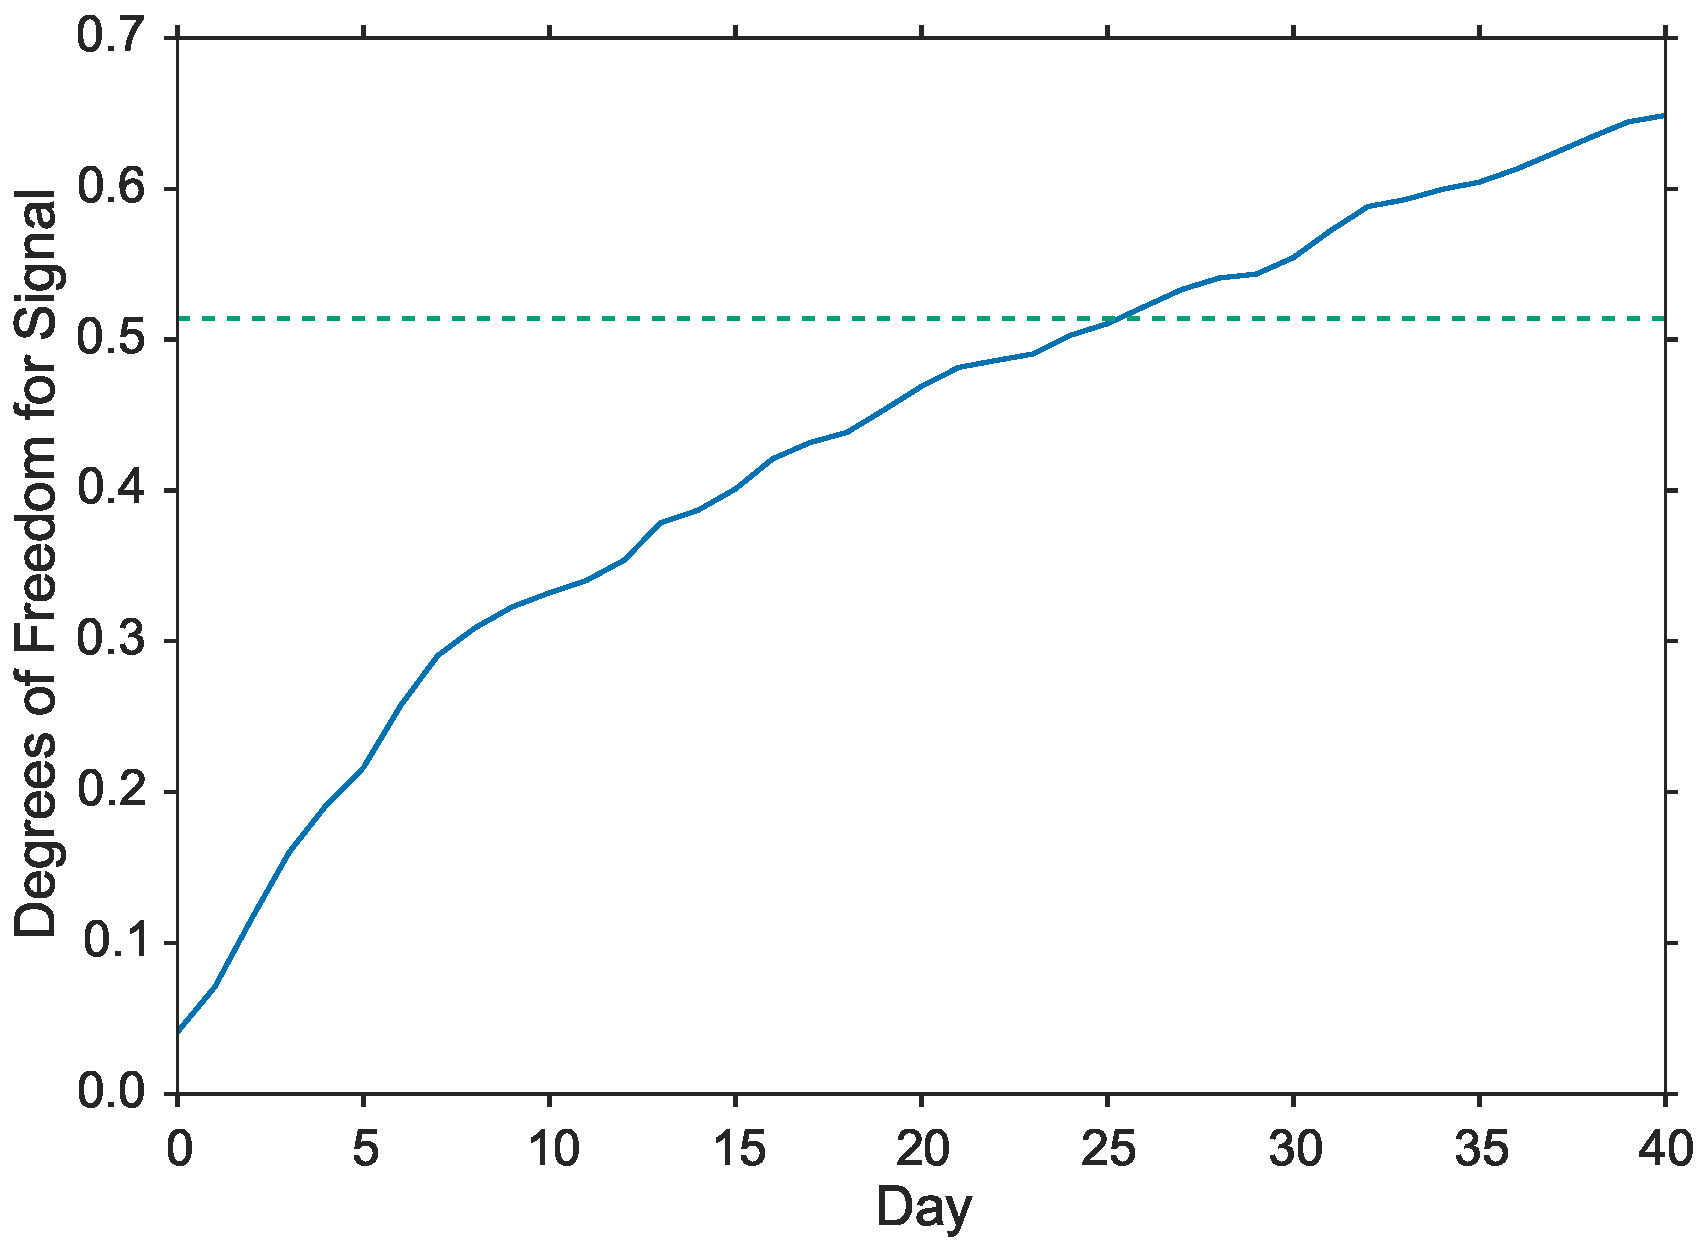
\includegraphics[width=\textwidth]{chapter/chapter5/dfs_succ_nee.pdf}
        \caption{\(dfs\) for successive NEE observations}
        \label{chap5:fig:dfs_succ_nee}
    \end{subfigure}
    \caption{Blue line: SIC and \(dfs\) for as successive NEE observations are added for 40 days from the \(1^{\text{st}}\) January 2007 using driving data from a pine stand in Oregon, green dotted line: SIC and \(dfs\) for a single summer observation of NEE made on \( 22^{\text{nd}} \) June 2007. }
    \label{chap5:fig:ic_succ_nee}
\end{figure}

\subsubsection{Effect of time correlations between observation errors on information content}

We can see the effect on the analytic representation of information content for two successive observations of NEE when including an off-diagonal correlation term in the matrix \(\hat{\mathbf{R}}\). So that \(\hat{\mathbf{R}} = \hat{\mathbf{D}}\mathbf{C}\hat{\mathbf{D}}^{\text{T}}\), where \(\hat{\mathbf{D}}\) is the diagonal matrix of observation standard deviations and \(\mathbf{C}\) is a correlation matrix of the same shape. We then have
\begin{equation}
\hat{\mathbf{R}} =  \hat{\mathbf{D}}\mathbf{C}\hat{\mathbf{D}}^{\text{T}} =
\begin{pmatrix}
\sigma_{nee,o} & 0  \\
0 & \sigma_{nee,o}  \\
\end{pmatrix}
\begin{pmatrix}
1 & \rho  \\
\rho & 1  \\
\end{pmatrix}
\begin{pmatrix}
\sigma_{nee,o} & 0  \\
0 & \sigma_{nee,o}  \\
\end{pmatrix}
=
\begin{pmatrix}
\sigma_{nee,o}^{2} & \rho\sigma_{nee,o}^{2}  \\
\rho\sigma_{nee,o}^{2} & \sigma_{nee,o}^{2}  \\
\end{pmatrix},
\end{equation}
with \(0 \leq \rho < 1\).

We have not shown the analytic representation for the SIC here as it is too large. We instead use the symbolic Python package SymPy \citep{Joyner:2012:OSC:2110170.2110185} to plot the SIC for an increasing value of \(\rho\) in figure~\ref{chap5:fig:sic_corr_D1}.
\begin{figure}[ht]
	\centering
        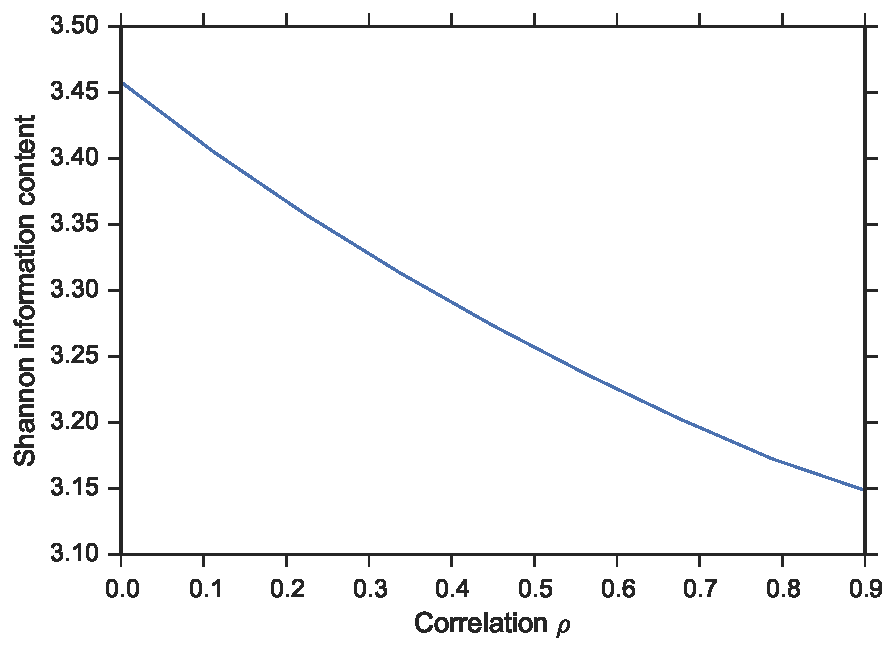
\includegraphics[width=0.5\textwidth]{chapter/chapter5/sic_corr_D1_nee.pdf}
    \caption{Shannon information content for two successive observations of NEE when a varying time correlation is included between observation errors.}
    \label{chap5:fig:sic_corr_D1}
\end{figure}
Figure~\ref{chap5:fig:sic_corr_D1} shows that as the size of time correlation \(\rho\) approaches 1 the information content in the two observations of NEE decreases. This decrease in information content makes sense as including the correlation in time is decreasing the amount of independent information we are assimilating. This result is also seen in \citet{jarvinen1999variational} where including a serial correlations between observation errors is shown to reduce the weight given to the mean of the observations in the assimilation (equivalent to inflating the variance of the observations). The effect of including correlations in time between NEE observation errors is further explored in chapter~\ref{chap:error_corrs}.

\subsection{DALEC2 information content for state and parameter estimation} \label{chap5:sec:D2_IC}%%%%%%%%%%%%%%%%%%%%%%%
\subsubsection{Information content in observations for DALEC2}
%SIC with D2 show same for single time, inf mat for evergreen and deciduous, difference in phenology has effect on info %content when model is involved successive obs less valuable than ones at start of the window. show col sums for inf mat.

In this section we repeat and extend some of the results we have found for information content with the DALEC1 state estimation case in section \ref{chap5:sec:D1_IC} to the DALEC2 joint parameter and state estimation case. This means we now have an augmented state of 23 elements (17 parameters and 6 state variables) as opposed to just the 5 state members for DALEC1. For this reason we no longer examine the analytic representations of information content but instead consider the information content calculated numerically for DALEC2. 

In section~\ref{chap5:sec:info_con_single_time} it was shown that for DALEC1 the information content for a single observation of NEE was dependent on temperature. From Figure~\ref{chap5:fig:neeSIC_temp_comp_D2} we can see that this is still the case for DALEC2. However the value of SIC is higher for DALEC2 in Figure~\ref{chap5:fig:neeSIC_temp_comp_D2} than for DALEC1 in Figure~\ref{chap5:fig:neeSIC_temp_comp} as the augmented state for the DALEC2 case also includes the parameters. This means that a single observation of NEE is giving us information about more elements of the state than for the DALEC1 state estimation case.

\begin{figure}[ht]
    \centering
    \begin{subfigure}[b]{0.45\textwidth}
        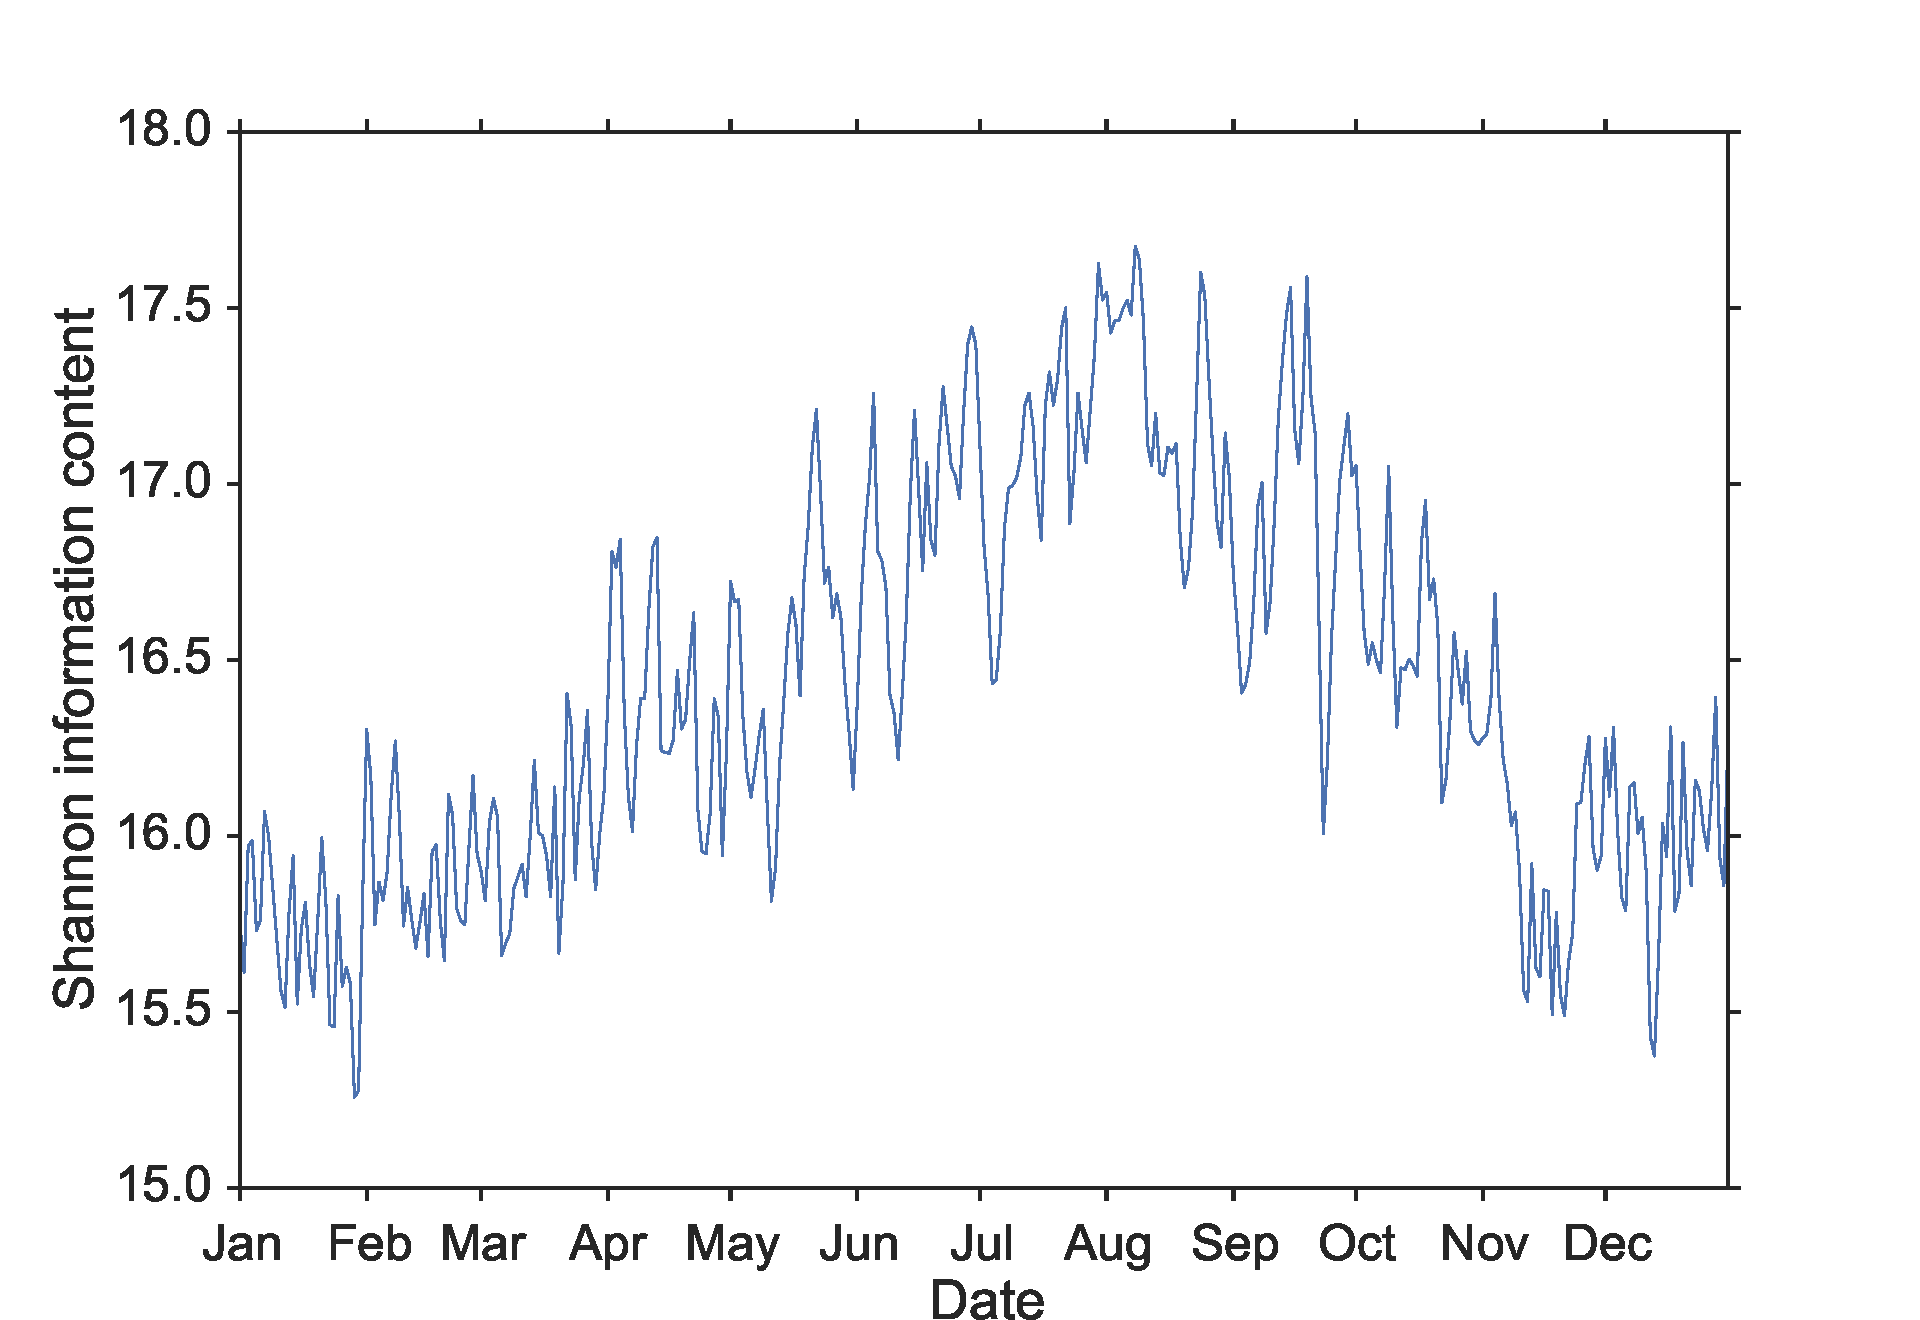
\includegraphics[width=\textwidth]{chapter/chapter5/oregon2007SICneeD2.pdf}
        \caption{SIC for single NEE observation}
        \label{chap5:fig:sic_nee_oregon2007_D2}
    \end{subfigure}%
    \begin{subfigure}[b]{0.45\textwidth}
        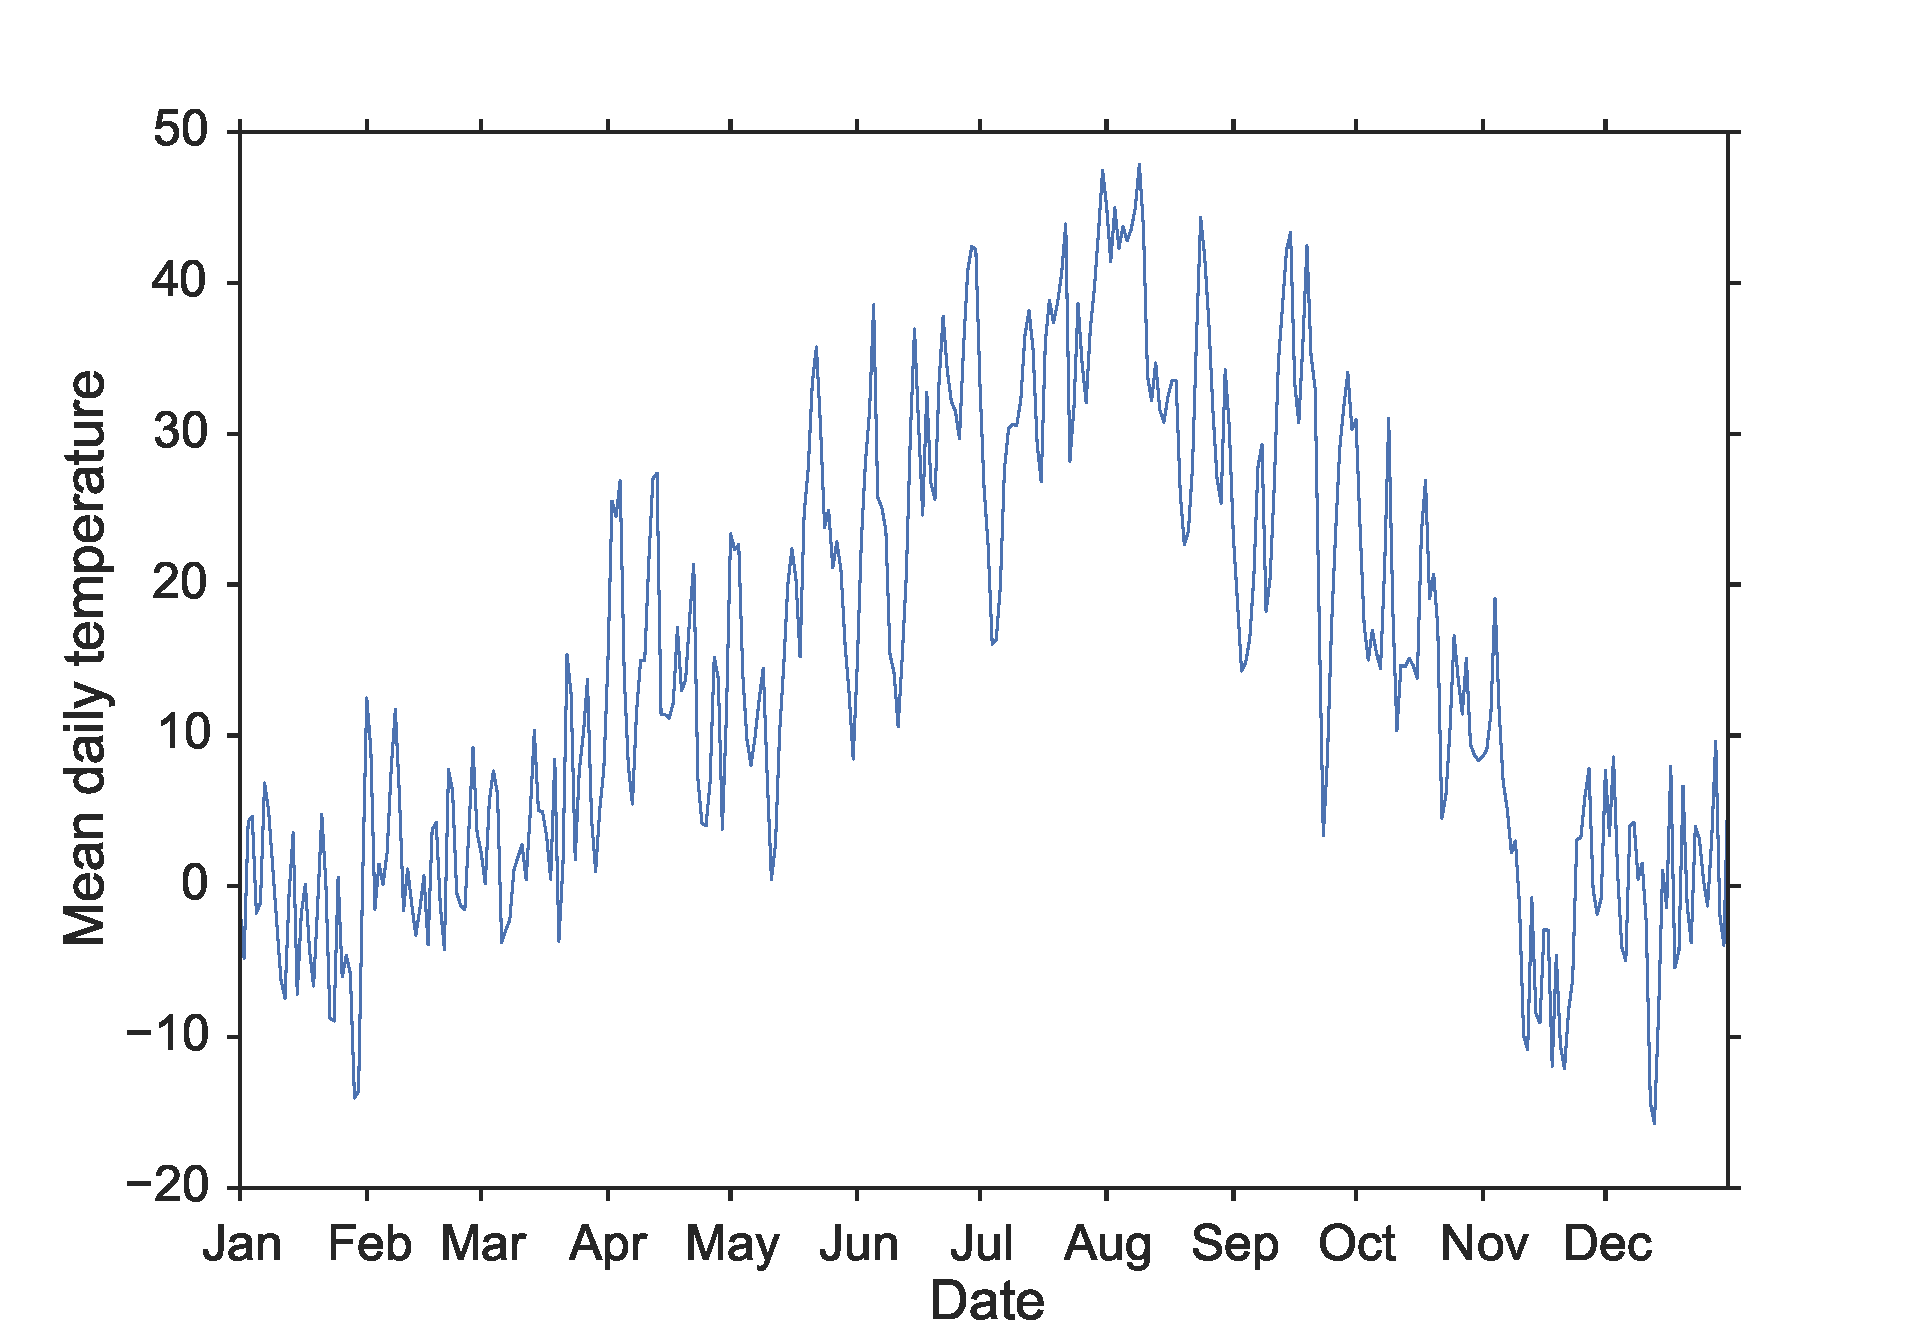
\includegraphics[width=\textwidth]{chapter/chapter5/oregon2007temp.pdf}
        \caption{Mean daily temperature for year's data}
        \label{chap5:fig:temp_nee_oregon2007_D2}
    \end{subfigure}
    \caption{SIC a single NEE observation changing throughout a year's window using driving data from a pine stand in Oregon taken in 2007 (left). Mean daily temperature for the same site and period (right).}
    \label{chap5:fig:neeSIC_temp_comp_D2}
\end{figure}

In figure~\ref{chap5:fig:neeSIC_temp_comp_D2} we have shown the information content varying for an evergreen forest site. As DALEC2 can also be parameterised and run for deciduous sites (with much work in this thesis being undertaken at Forest Research's deciduous study site, see section~\ref{chap4:sec:aliceholt}) it is important to investigate the difference in information content between these cases. In order to visualise this difference, in figure~\ref{chap5:fig:inf_mats} we show the analysis sensitivity to observations or influence matrix \citep{Cardinali2004} as described in section~\ref{chap5:sec:inf_mat}, \(\textbf{S} = \textbf{K}^{T}\textbf{H}^{T}\), for a year's assimilation window with 365 observations of NEE. The influence matrix will depend on the initial augmented state we chose to linearise around, the driving data we use to run our model and the observations we specify for assimilation. In figure~\ref{chap5:fig:inf_mats} we use an initial augmented state optimised for the Alice Holt deciduous forest and an initial augmented state optimised for an evergreen site in Oregon, we then use the same yearly driving data for both states so that it is only the difference between the initial augmented states of the sites effecting the difference between the influence matrices.  

\begin{figure}[ht]
    \centering
    \begin{subfigure}[b]{0.46\textwidth}
        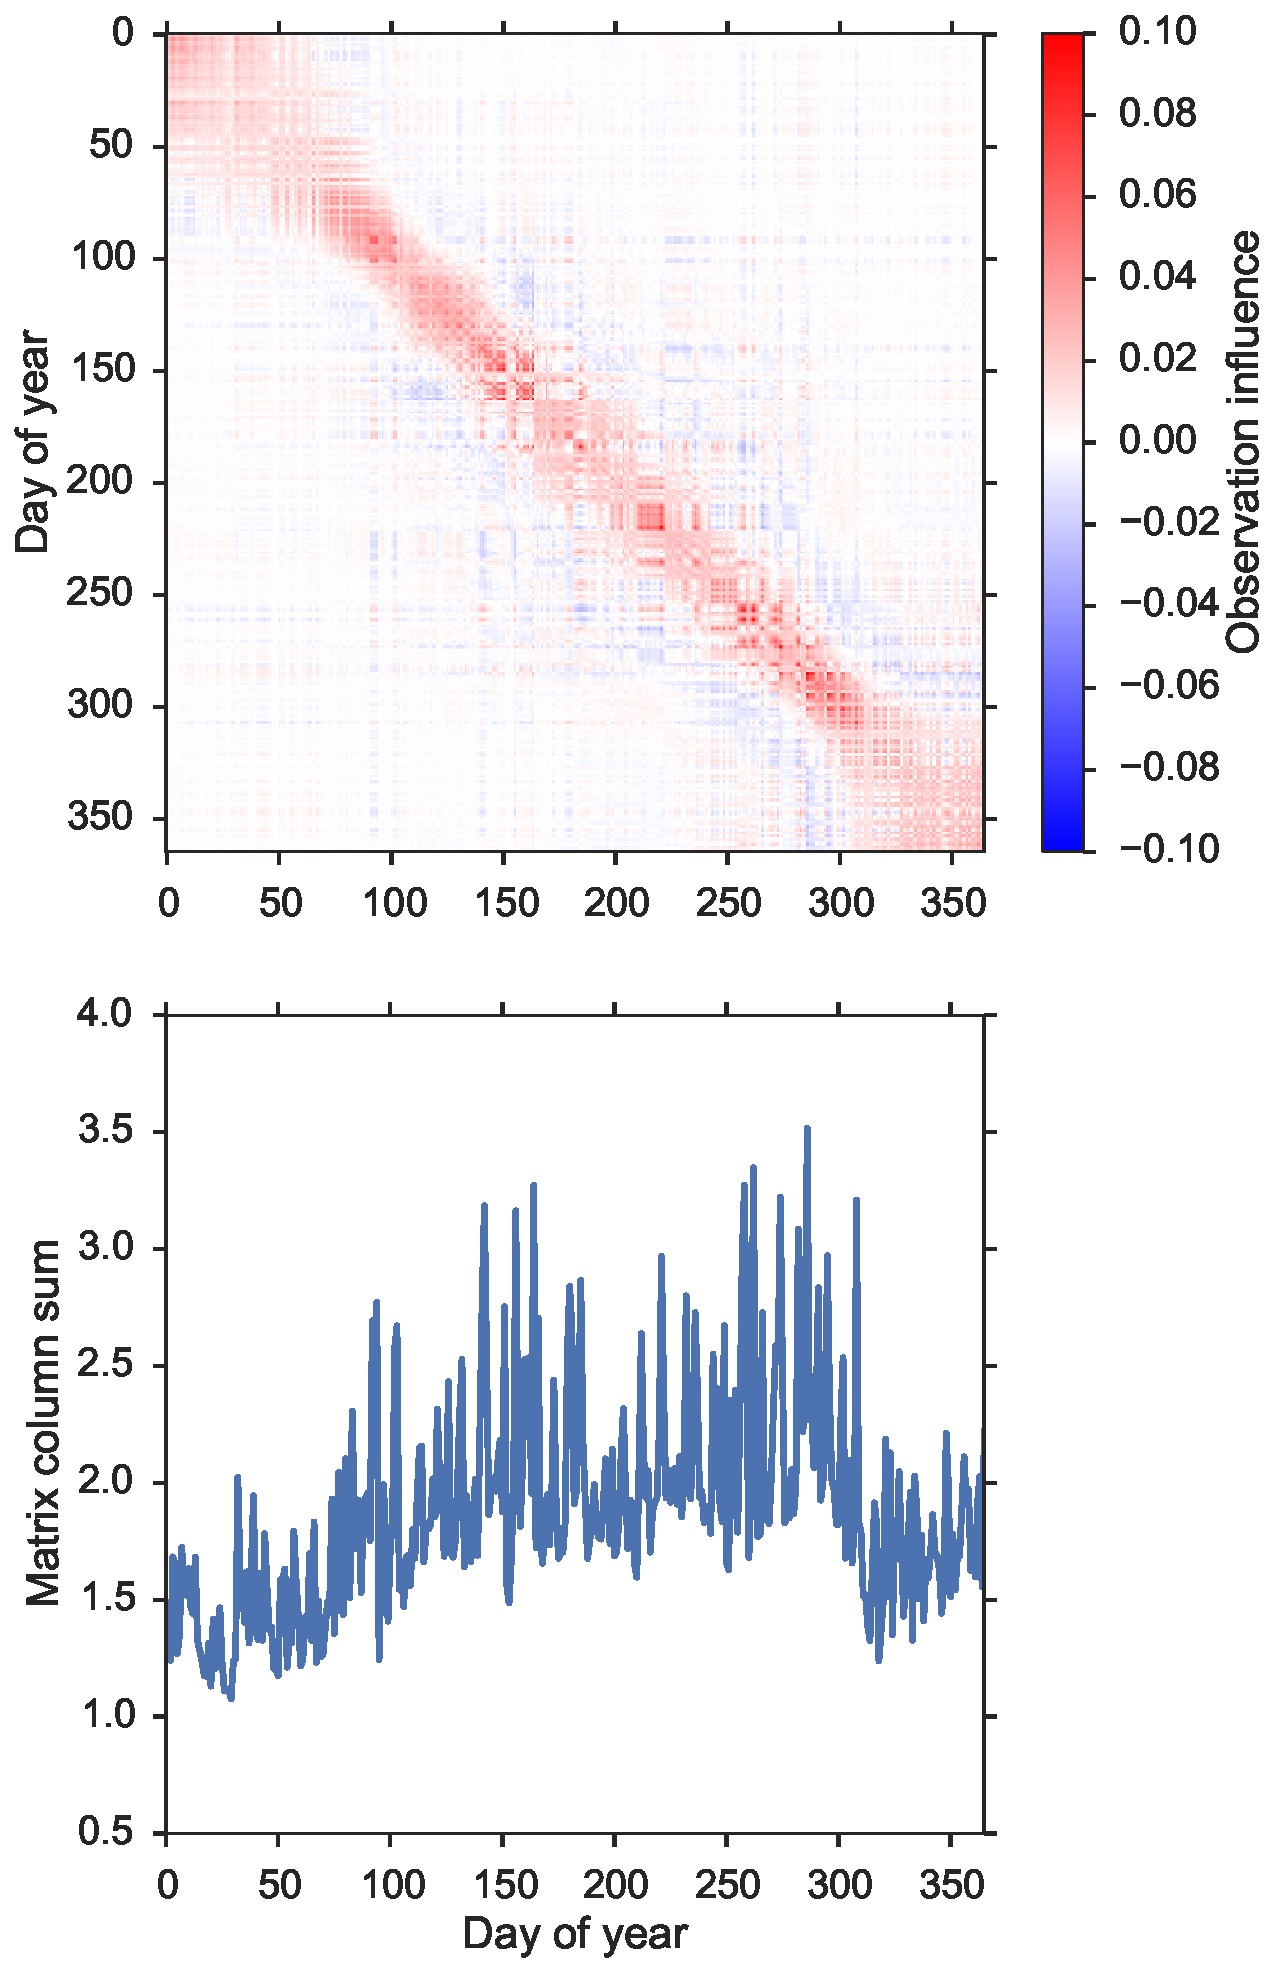
\includegraphics[width=\textwidth]{chapter/chapter5/inf_mat_sa.pdf}
        \caption{Alice Holt deciduous site}
        \label{chap5:fig:ah_inf_mat}
    \end{subfigure}%
    \begin{subfigure}[b]{0.46\textwidth}
        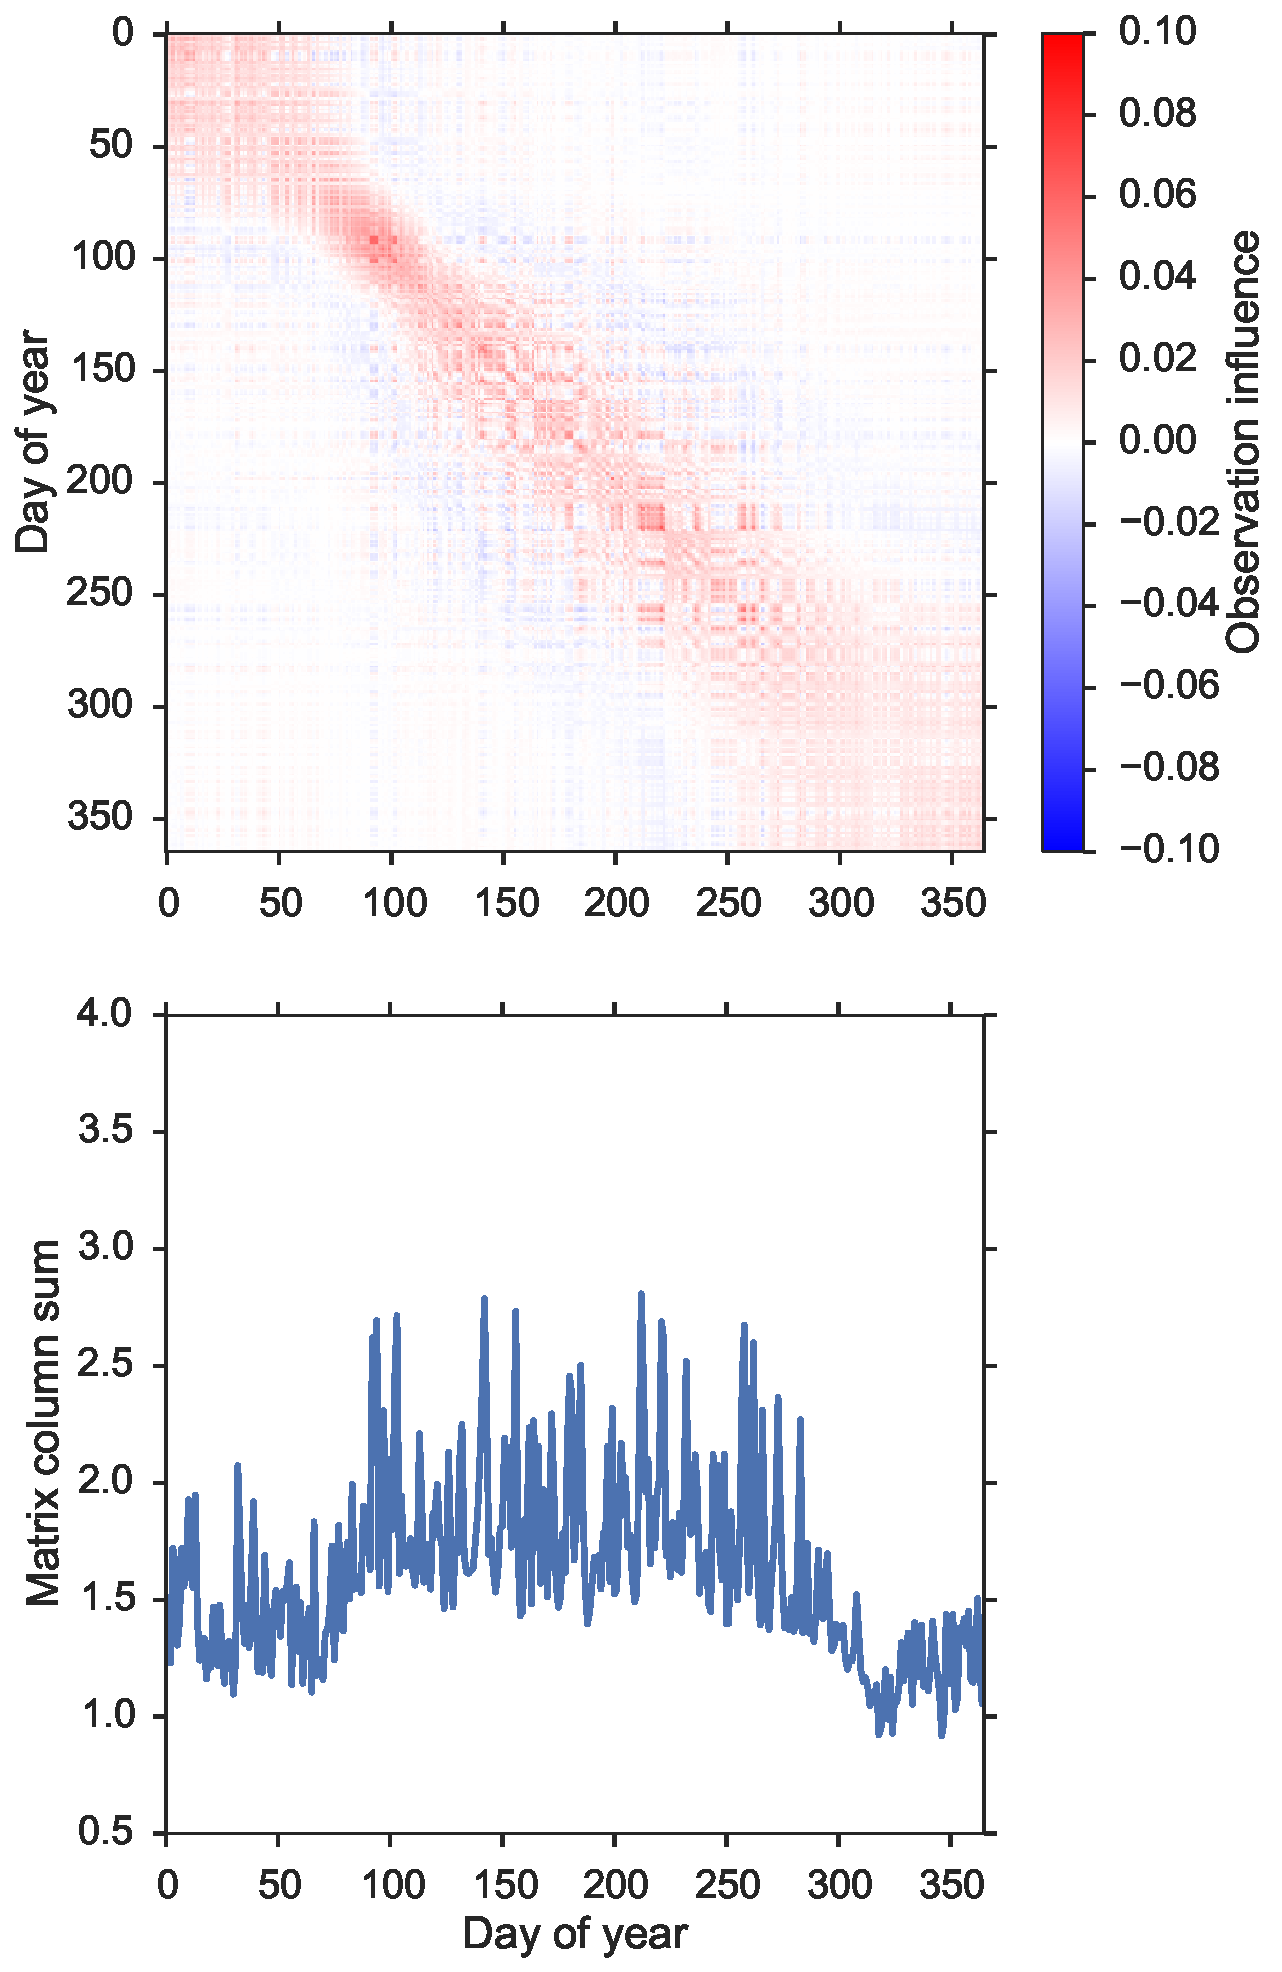
\includegraphics[width=\textwidth]{chapter/chapter5/inf_mat_so.pdf}
        \caption{Oregon evergreen site}
        \label{chap5:fig:oregon_inf_mat}
    \end{subfigure}
    \caption{Influence matrices and column absolute value sums as described in section~\ref{chap5:sec:inf_mat}, showing the sensitivity of the modelled observations to the assimilated observations for a year's assimilation window starting at the beginning of January with 365 observations of NEE.}
    \label{chap5:fig:inf_mats}
\end{figure}

From figure~\ref{chap5:fig:inf_mats} we can see that the influence of the assimilated observations of NEE is noticeably different between the deciduous and evergreen sites. However, in both cases at the beginning of the window there is a group of observations with similar influence. This makes sense as we are predicting the initial augmented state for DALEC2, so that observations closer to this initial state should have greater influence. 

For the deciduous site in figure~\ref{chap5:fig:ah_inf_mat} we have groups of observations with high influence from around day 125 to day 175 and from day 250 to day 300. We also have some high influence observations between these two groups. High influence observations between these two groups would be consistent with the results showing that NEE observations have higher information content with higher temperatures, as the period between day 175 and 250 contains days with higher mean temperatures. For the evergreen site in figure~\ref{chap5:fig:oregon_inf_mat}, although we have a group of observations at the beginning of the growing season with higher influence, we do not see a group of with the same high influence between day 250 to day 300 as with the deciduous case. We still see observations of high influence corresponding to times of higher temperatures for the evergreen case. 

\begin{figure}[ht]
    \centering
    \begin{subfigure}[b]{0.45\textwidth}
        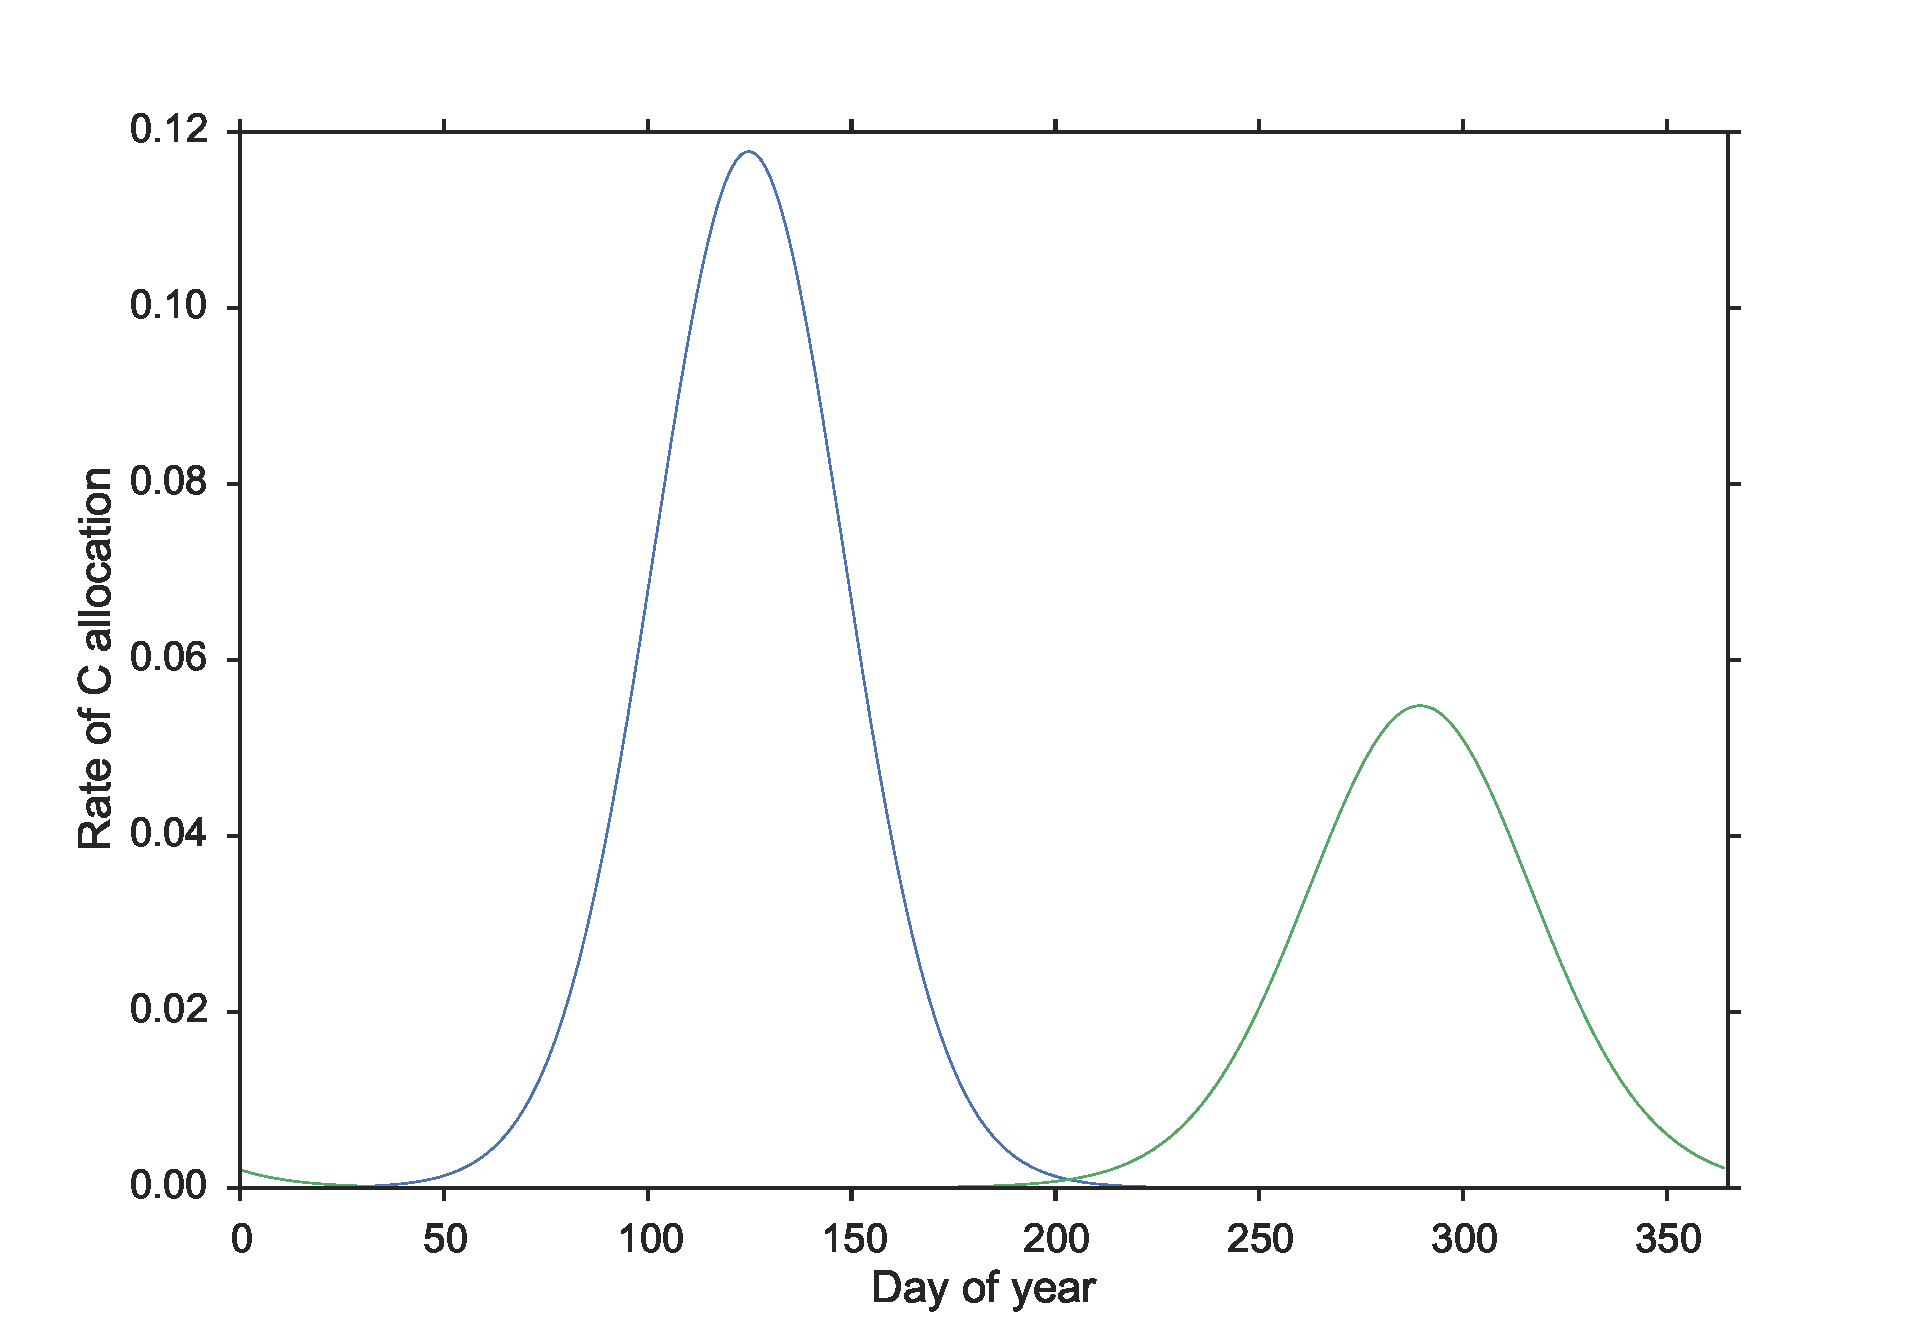
\includegraphics[width=\textwidth]{chapter/chapter5/ah_pheno.pdf}
        \caption{Alice Holt deciduous site}
        \label{chap5:fig:ah_pheno}
    \end{subfigure}%
    \begin{subfigure}[b]{0.45\textwidth}
        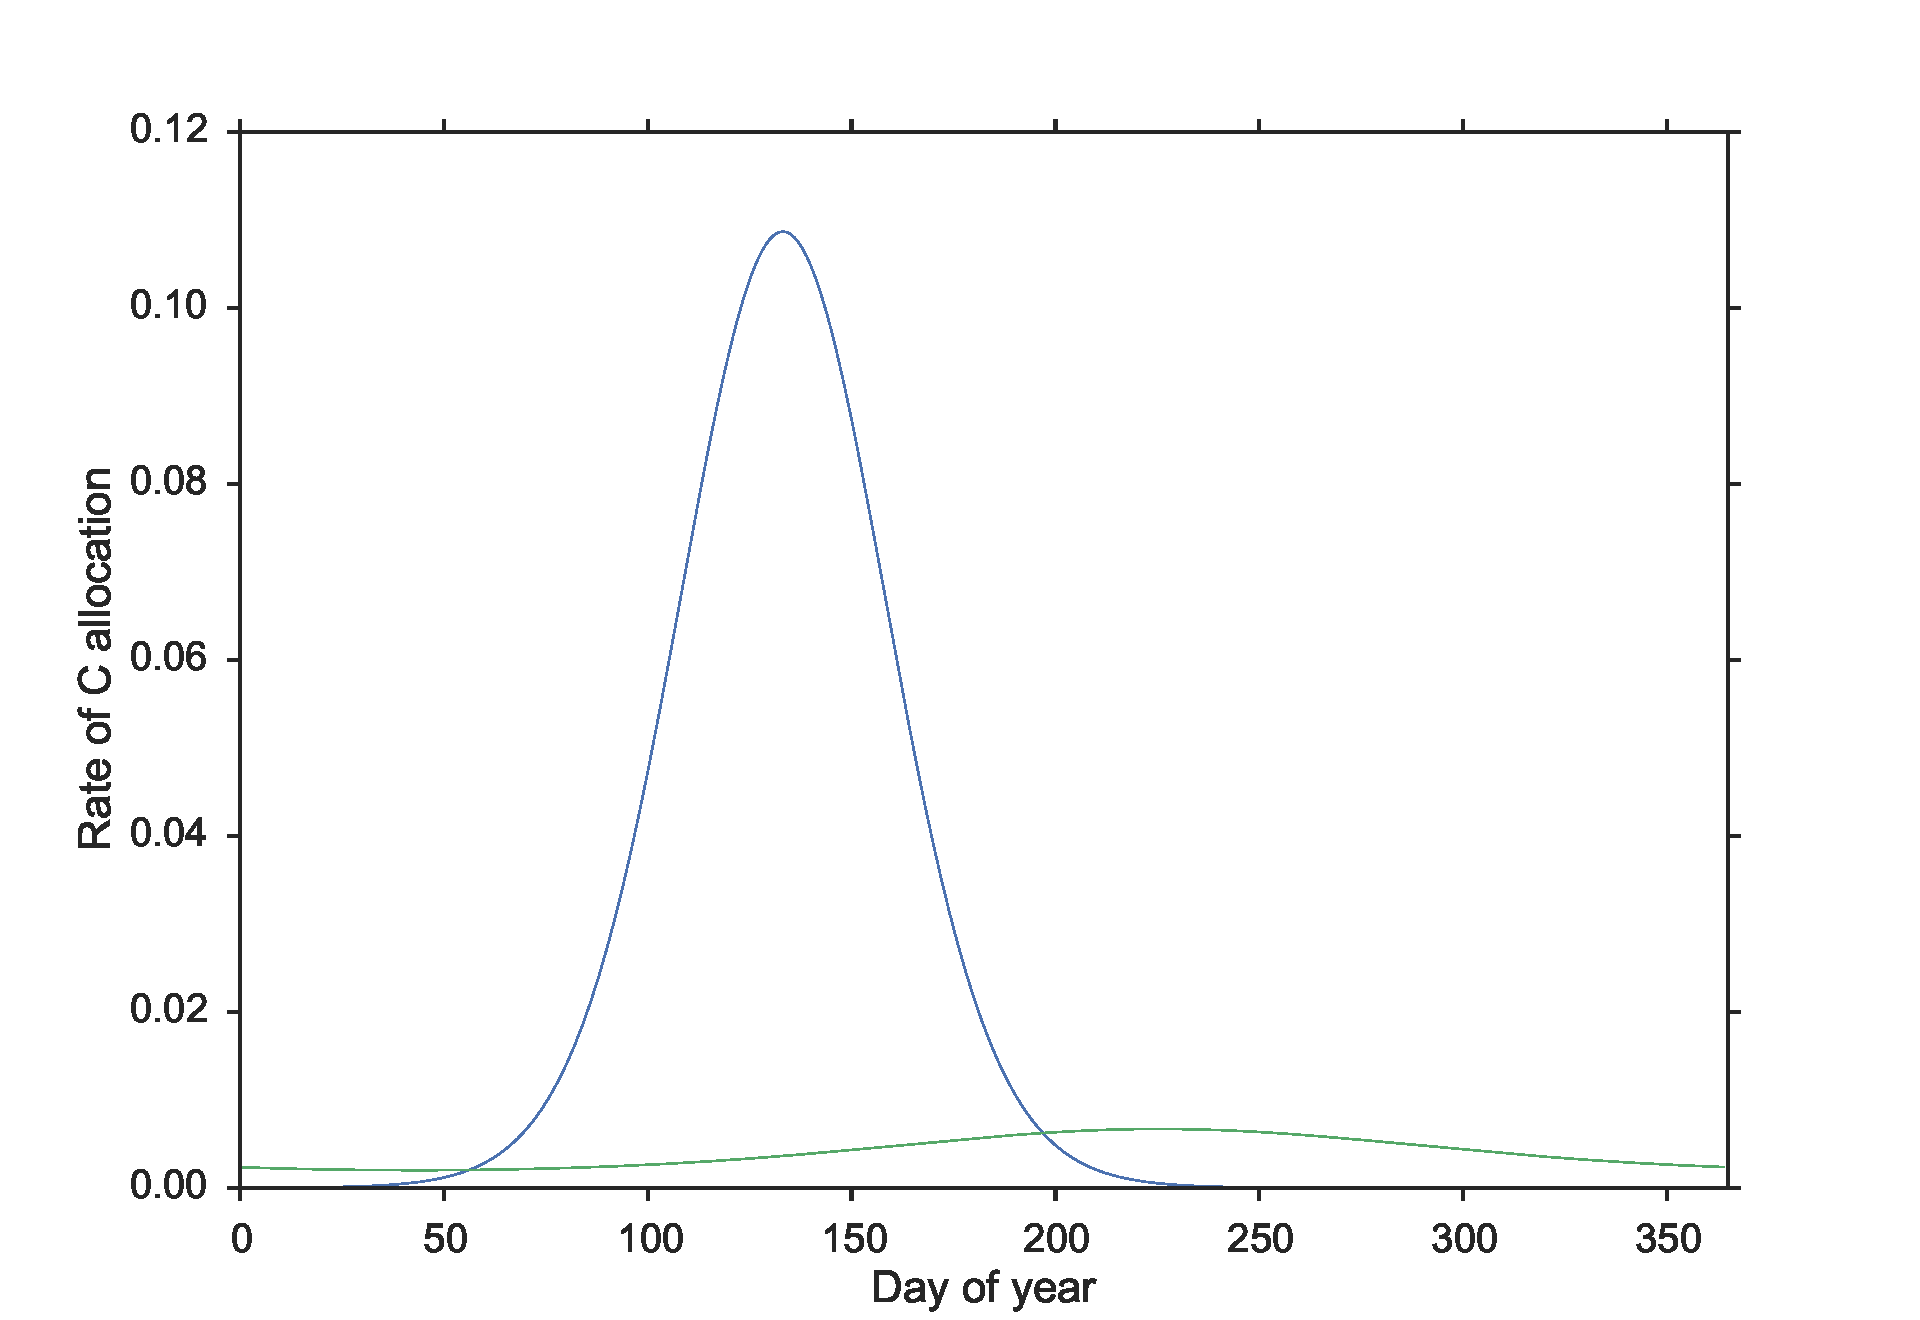
\includegraphics[width=\textwidth]{chapter/chapter5/oregon_pheno.pdf}
        \caption{Oregon evergreen site}
        \label{chap5:fig:oregon_pheno}
    \end{subfigure}
    \caption{Phenology of DALEC2 model for a deciduous and evergreen forest. Blue line: function controlling rate of leaf-on (\(\phi_{on}\)), green line: function controlling rate of leaf-off (\(\phi_{off}\)).}
    \label{chap5:fig:D2_pheno}
\end{figure}

In order to further investigate these groups of high influence observations we show the phenology functions controlling the rate of leaf-on and leaf-off for the DALEC2 model in figure~\ref{chap5:fig:D2_pheno}. The description of phenology is the main difference between the more simplistic, evergreen only, DALEC1 and DALEC2 which can be parameterised for both deciduous and evergreen sites. It is logical that this is what is causing the difference in information content between the models and between the different sites. In figure~\ref{chap5:fig:D2_pheno} we see that the function controlling leaf-off for the deciduous site has a far larger peak than that of the evergreen site. This is expected as the deciduous site will drop all of its leaves at the end of the season. In both cases the forest puts most effort into putting on new leaves at the start of the growing season. This highlights the fact that the NEE for a deciduous site is highly controlled by phenology, as the forest cannot photosynthesise without leaves. Therefore the observations of NEE that help to constrain the phenology of the site should have a higher influence, as seen in figure~\ref{chap5:fig:ah_inf_mat}. Conversely for an evergreen site NEE is driven less by phenology and more by the climatic driving data. Seeing a greater relationship between temperature and information content  for an evergreen site consequently makes sense and this can be seen in figure~\ref{chap5:fig:oregon_inf_mat}.



\subsubsection{Effect of time correlations on observation information content}

In section~\ref{chap5:sec:D1_succ_obs} it was shown that, for the analytic DALEC1 case, when assimilating two successive observations of NEE the SIC decreased when including a correlation in time between NEE observation errors. It was noted that this was consistent with results found in \citet{jarvinen1999variational} where including correlations between observation errors in time reduced the weight of the observations in the assimilation. In figure~\ref{chap5:fig:sic_corr_D2} we repeat the experiment in section~\ref{chap5:sec:D1_succ_obs} but for the DALEC2 joint parameter and state estimation case with NEE observations for the year 1999 from the Alice Holt flux tower site, in order to verify that including a correlation in time reduces the information content in assimilated observations. 
\begin{figure}[ht]
	\centering
        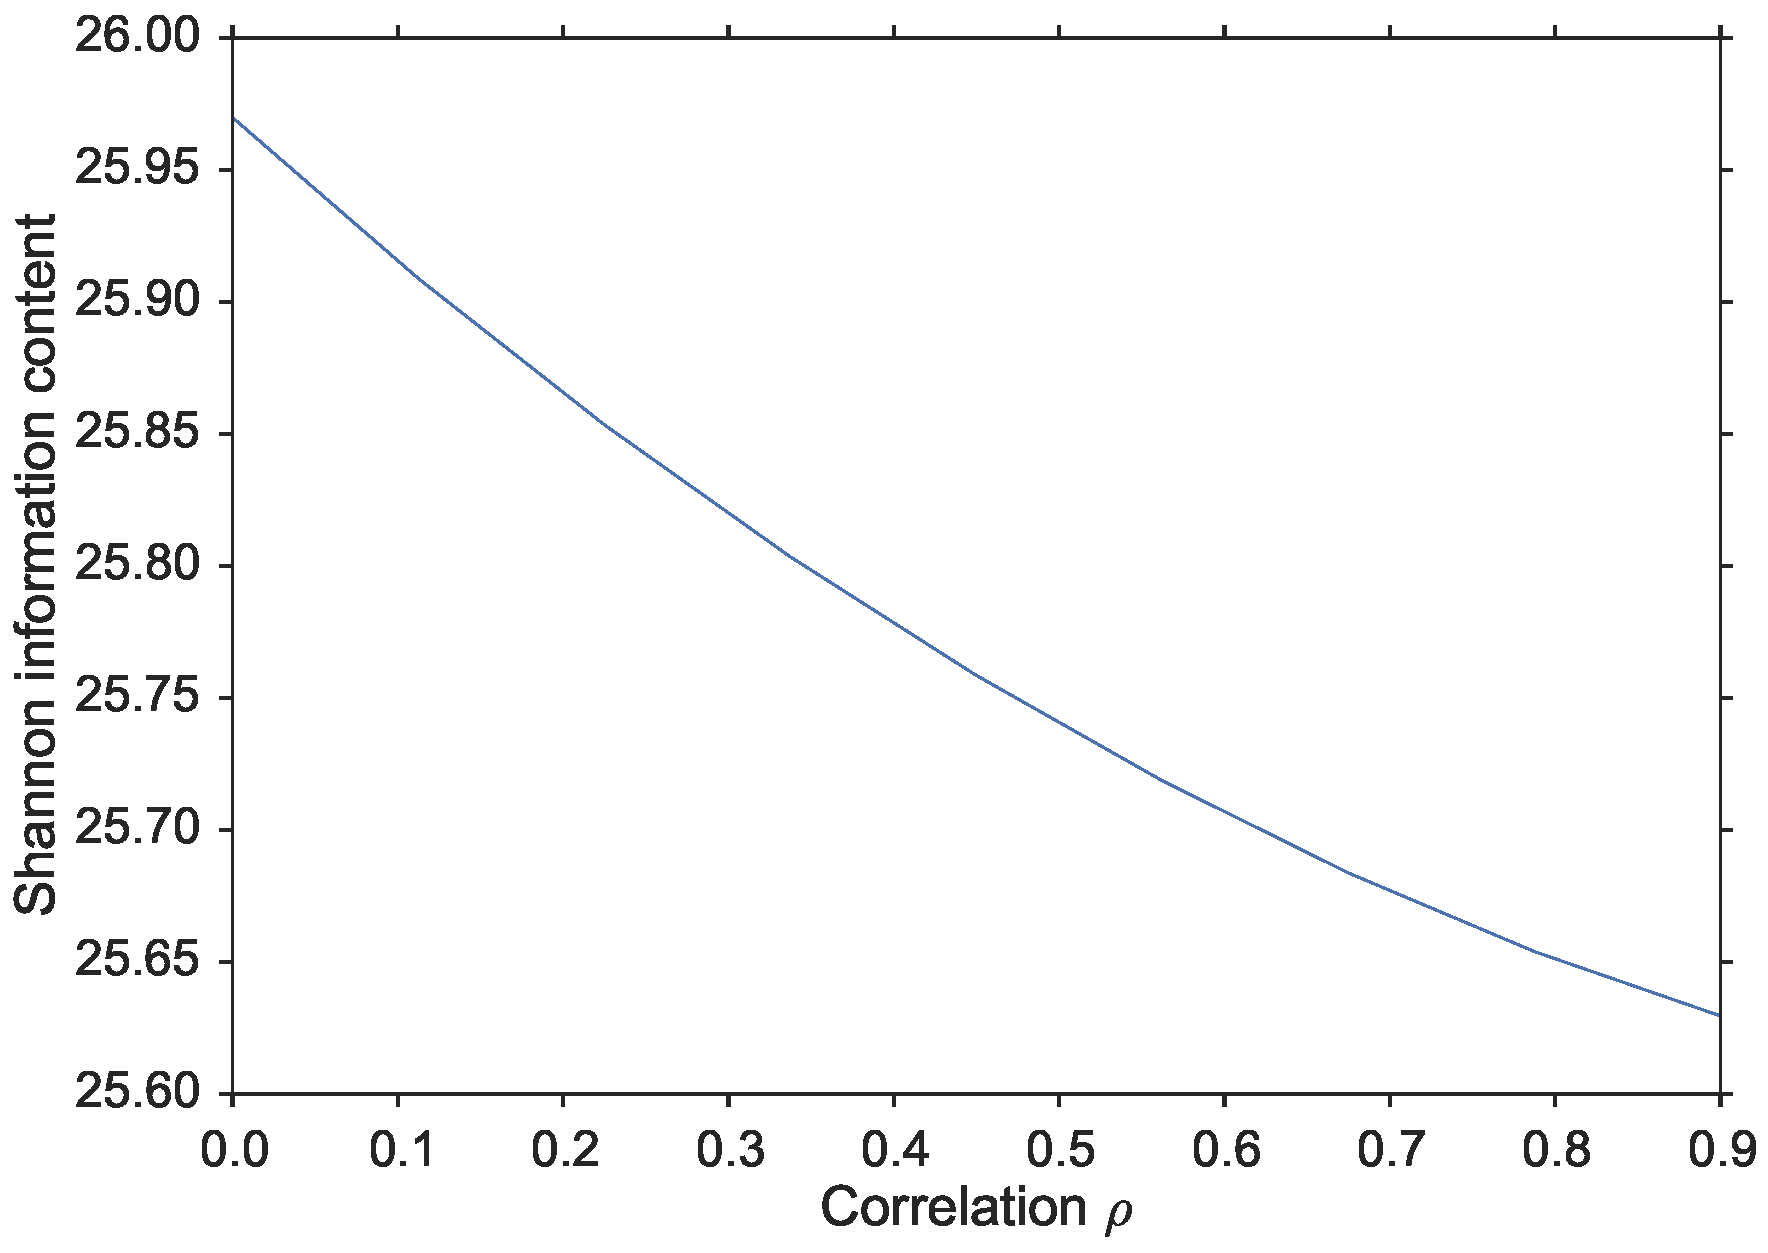
\includegraphics[width=0.5\textwidth]{chapter/chapter5/sic_corr_D2_nee.pdf}
    \caption{Shannon information content for 67 observations of NEE taken throughout a year's assimilation window when a varying time correlation is included between observation errors.}
    \label{chap5:fig:sic_corr_D2}
\end{figure}
From figure~\ref{chap5:fig:sic_corr_D2} we see that we have similar results as in figure~\ref{chap5:fig:sic_corr_D1} where the information content in our observations decreases as we increase the time correlation between the assimilated observation errors. However, in figure~\ref{chap5:fig:sic_corr_D2} we have a higher value of SIC as we are assimilating many more observations than in figure~\ref{chap5:fig:sic_corr_D1}. In figure~\ref{chap5:fig:sic_corr_D2} we have used the same correlation function as in section~\ref{chap6:sec:corR} to create a correlated matrix \(\hat{\textbf{R}}\) and then varied the magnitude of the included correlation, \(\rho\). The decreasing information content with an increasing correlation between observation errors in time supports the results in section~\ref{chap5:sec:D1_succ_obs}. This is also consistent with the results of \citet{jarvinen1999variational} where including correlations between observation errors in time is shown to reduce the weight given to the mean of the observations in the assimilation (equivalent to inflating the variance of the observations). The effect of these temporal error correlations is invertigated further in chapter~\ref{chap:error_corrs}. 

%\subsubsection{Increasing available information by day/night sampling of NEE}

%In previous work we have averaged the 48 half-hourly measurements of NEE in a day to find a value for total daily NEE. This is because we are working with a model that has a daily time step and thus need to assimilate observations at the same temporal resolution. In REF Richardson et al... it is shown that the assimilation of NEE averaged half daily (so that we have observations of daytime NEE and nighttime NEE) can improve data assimilation results and the model partitioning between GPP and RT. This is because nighttime NEE is equal to RT as no photosynthesis occurs at night.

%In this section we will show how we can assimilation day and nighttime NEE without making any modifications to our model. We do this by creating two modified observation operators to relate our model state and parameters at time \(i\) to both daytime and nighttime NEE at time \(i\). We still use the DALEC2 model here but this technique is applicable to any other ecosystem carbon model. Here we show a set of twin experiments to illustrate how assimilating NEE twice daily can be beneficial over assimilating a single value of total daily NEE. The main benefit coming from the fact that we have a greater number of observations after processing the raw eddy covariance data. This is because we are averaging over fewer half-hourly observations so have a lower probability of gaps appearing in our averaging period. This means we throw away less observations than we would when averaging over the total 48 half-hourly observations of NEE in a day.

\section{Conclusions}

In this chapter we have investigated both the observability and information content given the observations available to us. In section~\ref{chap5:sec:D1observability} and section~\ref{chap5:sec: D2_observability} we have shown that for both DALEC1 and DALEC2 we have an observable system with the available observations, in this case NEE. An observable system in this case means that for data assimilation we can construct a locally unique solution from the observational information alone. 

In section~\ref{chap5:sec:D1_IC} we have seen that for the DALEC1 evergreen case the information content in observations of NEE is largely dependent on temperature, with higher temperatures meaning higher information content. This is important for informing planned maintenance or down time at flux tower sites measuring NEE. This dependance of information content on temperature is also seen for observations of ground respiration and total ecosystem respiration. When assimilating additional observations at the same time alongside NEE we have found that most information is added when the additional observation provides an orthogonal constraint to that of NEE. This is the case for root carbon (\(C_{roo}\)) and woody biomass carbon (\(C_{woo}\)), with the European Space Agency BIOMASS mission being launched soon this should add valuable information to current data assimilation schemes. When using DALEC1 and assimilating successive observations in time it was shown that as observations are added further away from the initial state their impact is decreased. For two successive observation of NEE it was also shown that including a correlation in time between observation errors decreases the information content in the assimilated observations. This is consistent with results found in \citet{jarvinen1999variational} where including correlations between observation errors in time is shown to reduce the weight given to the mean of the observations in the assimilation.

In section~\ref{chap5:sec:D2_IC} we again see the temperature dependence of information content in observations of NEE for DALEC2. However, for DALEC2 we also have varying information content based on the type of ecosystem we are observing. For a deciduous forest site we see that as well as temperature the information content in observations of NEE is strongly dependent on the time of growing season. Observations made at the time of leaf-on and leaf-off have higher influence on the results of the assimilation. This makes physical sense as for a deciduous ecosystem NEE is highly controlled by phenology, as the forest cannot photosynthesise without leaves. Therefore the observations of NEE that help to constrain the phenology of the site should have a higher influence. For an evergreen forest site we see much less dependence on phenology and have a greater relationship between temperature and information content. We again see similar results as in section~\ref{chap5:sec:D1_IC} when including correlations in time between observation errors, with an increasing correlation, \(\rho\), reduces the information content in the assimilated observations.
